\documentclass[11pt,a4paper]{article}
\usepackage[margin=2.5cm]{geometry}
\usepackage{amsmath,amssymb}
\usepackage{graphicx}
\usepackage[export]{adjustbox}
\usepackage{booktabs}
\usepackage{longtable}
\usepackage{tabularx}
\usepackage{xcolor}
\usepackage{tcolorbox}
\tcbuselibrary{breakable}
\usepackage{enumitem}
\usepackage{microtype}
\usepackage{needspace}
\usepackage{url}
\urlstyle{tt}
\emergencystretch=2em
\definecolor{labblue}{HTML}{1F4E79}
\widowpenalty=10000
\clubpenalty=10000
\setlength{\parskip}{0.35em}
\usepackage[colorlinks=true, linkcolor=labblue,
            citecolor=labblue, urlcolor=labblue, bookmarks=true,
            bookmarksnumbered=true, unicode=true]{hyperref}
\begin{document}
\begin{center}
{\huge\bfseries\color{labblue} The Dirac Skeleton of the AB-Cloud}\\[0.8em]
{\large A numerical laboratory connecting the Hofstadter-vortex realization of the Hilbert-Polya programme to the Dirac equation}\\[1.2em]
{\normalsize Isaev Iskhak Khamzatovich}\\[0.3em]
{\small ORCID 0009-0003-7299-0701 --- Independent Researcher --- AB-Cloud Research Programme}\\[0.3em]
{\small October 2026}
\end{center}
\begin{tcolorbox}[breakable, colback=labblue!6, colframe=labblue!70!black, boxrule=0.6pt, title={Abstract / Аннотация}]
The parent AB-Cloud programme constructs a Hofstadter Hamiltonian decorated with topological vortices whose Aharonov-Bohm phases encode the non-trivial zeros of the Riemann zeta function, and verified that at the self-dual flux alpha = 1/2 the system exhibits Dirac dynamics (E\_\allowbreak{}min proportional to 1/L, R-squared = 0.9997). This monograph takes that observation seriously and develops it into a complete lattice-Dirac laboratory of eight verification tests (D1-D8). We prove numerically that the clean alpha = 1/2 Hofstadter model IS a lattice discretization of the massless Dirac equation: the Bloch bands match the analytic pi-flux dispersion to 2.7e-15, the Fermi velocity extracted from the finite-size scaling is v\_\allowbreak{}F = 1.935 in units of the lattice hopping (continuum prediction v\_\allowbreak{}F = 2t, parent-suite fit v\_\allowbreak{}F = 1.9447), and the first Dirac level obeys E\_\allowbreak{}1 x L -> 2*pi*v\_\allowbreak{}F = 4*pi with 0.8 percent accuracy. The fourfold zero-mode tower is shown to be the Dirac zero mode structure on the torus with exact sublattice (chiral) polarization balance; a Wilson loop around the cone returns the Berry phase gamma = pi to twelve decimal places; a uniform field deviation produces the relativistic Landau ladder E\_\allowbreak{}n-squared proportional to n (R-squared = 0.99985-0.99999) together with the chiral n = 0 level pinned at E = 0, in sharp contrast to the Schrodinger ladder E\_\allowbreak{}n = B(n + 1/2) fitted to the same control operator. Real-time simulations reproduce Klein tunneling (normal-incidence transmission T = 0.978 through a barrier that suppresses the Schrodinger control to T = 0.0010, a factor of 977) and Zitterbewegung at omega = 2E (measured/theory = 0.99958 in a Dirac box and 0.9998 on the torus itself). The bridge test D7 decorates the Dirac lattice with vortex phases whose positions are deterministically coded from the first zeta zeros: the chiral skeleton survives exactly (\{H, Gamma\} = 0 and E <-> -E pairing to 4e-15), the level-ratio statistic moves from the GOE ceiling toward the GUE value 0.5992 (mean ratio r: 0.41-0.52 clean -> 0.605-0.608 decorated), while the exact four-tower splits into +-E valley pairs - an honest negative result whose mechanism (vanishing index, valley mixing) we establish in test D8. We conclude that the Dirac operator is the relativistic skeleton of the AB-cloud: the zeta-zero phases act as a topologically safe complexifier that unlocks GUE statistics without destroying the relativistic structure that the Hilbert-Polya programme requires. The v1.1 extensions implement the two development directions proposed in the first edition. Test D9 (index restoration) shows that a Jackiw-Rebbi mass domain wall binds chiral-pair quasi-zero modes pinned 4x10\^{}8 below the bulk gap of the grid Dirac operator; that the wall mode survives unchanged inside the full zeta-vortex background - the restoration contrast over the wall-less control is 7x10\^{}6; and that the full composite Jackiw-Rossi vortex (mass winding nu plus the statistical Goldstone flux nu/2) collapses the low-energy kernel to machine zero. Test D10 (Montgomery in motion) verifies the Montgomery pair correlation of the unfolded zero sequence (g(0.3) = 0.19 against theory 0.26 and the Poisson value 1; number variance 60x below Poisson) and demonstrates dynamically that GUE repulsion protects transport: the zeta-encoded vortex cloud reflects least and transmits most among equal-density configurations, with the Poisson cloud and the periodic cloud ordered in between. The zeta phases, the Dirac skeleton and the Montgomery statistics of the zeros are thus connected in both directions: the spectrum carries the zeros, and the dynamics carries the statistics. The v1.2 extension implements the last of the three proposed directions - the conjugation-action encoding of the zeros suggested by Berry-Keating and Connes. Test D11 realizes the cutoff dilation generator exactly on a log-coordinate lattice (arithmetic spectrum to 1.7e-13, exact conjugation algebra, exact Dirichlet trace comb of period Lambda), proves the recognition identity - the AB-Cloud coding phase t/delta is the fractional Berry-Keating staircase, to 4.6e-13 - verifies on the real zeros that the cutoff staircase tracks the Riemann counting to +-2.3 zero units with the 7/8 + <S> offset, shows that the transport protection survives the Connes substitution of the coding function (transmission 1.65x over Poisson; equivalence with the plain coding to 1.4 percent), and reads the zeros as the absorption spectrum of the conjugation drive: the drive form factor follows the GUE ramp on tau <= 0.75, and the protected-transport class persists along the whole dilation orbit. All eleven tests - 67 checks - pass in the canonical run; the D11 operator block is cross-verified in Julia. The v1.3 extensions move beyond the monograph's own Section 8 and close its natural continuations. Test D12 pushes the Berry-Keating ladder to the infinite limit at fixed spectral density: the trace comb sharpens into the delta train of the Connes/Weil trace formula (coherent peak N\_\allowbreak{}u exactly, off-peak envelope 1/(N\_\allowbreak{}u sin(pi/20)) down to 1.9e-4 at N\_\allowbreak{}u = 32768), the fixed-density staircase stays an exact integer identity at every band size, the extending band swallows the whole real-zero window, and the zeta protection proves extensive - the GUE statistics are lattice-size independent at fixed vortex density 25/900 while the encoded ladder grows from 25 to 64 vortices. Test D13 pairs the two previous extensions: the Jackiw-Rossi wall rides the physical Connes orbit pinned at |E\_\allowbreak{}0| = 3.9e-9 (profile fidelity 0.9999, contrast 7e6 along the whole orbit), while the conjugating generator lifts the valley multiplet only to a quasi-zero band at gap/679 - through an explicitly measured chiral breaking \{H(lambda), Gamma\} = lambda\{V, Gamma\}. Test D14 measures the second (two-point) form factor a la Odlyzko on three real-zero bands including a genuinely large-height band of 2000 zeros at t \textasciitilde{} 10\^{}5 from the official zeros6 table: the hard core K(0.1) <= 0.008, the GUE ramp K(0.25) = 0.123 < K(0.5) = 0.396, and the unit plateau already exact at t \textasciitilde{} 10\^{}5 (K(2) = 0.962), with the honest deviations (the tau = 1 estimator string, the band-specific K(0.25) elevation) documented. All fourteen tests - 96 checks - pass in the canonical run; the D12-D14 blocks are cross-verified in Julia.
\end{tcolorbox}
\tableofcontents
\newpage
\section{1. Introduction: from a phase resonator to the Dirac equation}
The Hilbert-Polya conjecture proposes that the non-trivial zeros of the Riemann zeta function are the spectrum of a self-adjoint operator. The AB-Cloud programme of the parent repository turns this proposal into an explicit lattice construction: a Hofstadter Hamiltonian on an L x L lattice, threaded by a uniform Aharonov-Bohm flux alpha per plaquette and decorated with topological vortices whose charges and phases are derived from the non-trivial zeros rho\_\allowbreak{}k = 1/2 + i t\_\allowbreak{}k of zeta(s). The parent verification suite (37 tests, two passes, ten independent language ports) established that this object reproduces GUE random-matrix statistics, is statistically indistinguishable from the zeta zeros themselves in the Montgomery test, and - decisively for the present work - exhibits Dirac dynamics at the self-dual flux alpha = 1/2: the minimal excitation scales as E\_\allowbreak{}min proportional to 1/L with R-squared = 0.9997, the density of states develops a deep dip at zero energy, and a fourfold zero-mode tower sits at machine-precision E = 0.

A scaling law E proportional to 1/L is the unmistakable fingerprint of a relativistic dispersion relation. For a massive (non-relativistic) particle the low-lying levels on a box of size L approach a constant; only a linear dispersion E = v\_\allowbreak{}F|k| produces E proportional to 1/L. The parent suite recorded the fingerprint but did not unpack it. This monograph unpacks it. We ask, and answer quantitatively, four questions. First, is the alpha = 1/2 Hofstadter model exactly a lattice Dirac equation, and what is its continuum limit? Second, what is the topological content of its zero modes - are they protected, and by what? Third, does the real-time physics of the lattice match the celebrated relativistic phenomena - Klein tunneling and Zitterbewegung - quantitatively? Fourth, and central to the AB-Cloud programme: what happens to this Dirac skeleton when it is decorated with the zeta-zero phases that define the AB-cloud?

The answers are delivered by an eleven-test verification suite (D1-D11) written in the parent repository's own culture: single-file, dependency-light, deterministic (seed 96), with explicit PASS/FAIL verdicts, per-test CSV artifacts, 600-dpi publication figures, and a full independent cross-implementation in Julia whose results agree with the canonical Python suite to LAPACK precision. All tests pass in the core run; the extension tests D9-D11 pass in full as well (Section 9 reports 10/10 checks, Section 10 reports 9/9, Section 11 reports 15/15). The headline numbers are: v\_\allowbreak{}F = 1.9347 extracted from the finite-size fit against the continuum prediction v\_\allowbreak{}F = 2t (the parent suite's own Test 30 reports 1.9447); a Berry phase of exactly pi around the cone; a relativistic Landau ladder with R-squared between 0.99985 and 0.99999 that beats the Schrodinger (linear-in-n) fit on the same operator; Klein transmission T = 0.9777 at normal incidence through a classically forbidden barrier that transmits only T = 0.0010 of the Schrodinger control; Zitterbewegung frequencies matching 2E to 4 decimal places; and a zeta-decoration that lifts the level-ratio statistic from the GOE ceiling to the GUE value 0.6080 at L = 48 (GUE theory 0.5992) while preserving the chiral skeleton to machine precision. The v1.2 conjugation-action test D11 closes the \S{}8 programme on the same lattice: the cutoff dilation generator of Berry-Keating is exact to 1.7e-13, the AB-Cloud coding phase is identified with the fractional Berry-Keating staircase to 4.6e-13, the GUE transport protection survives the Connes re-coding, and the drive form factor follows the GUE ramp.

The structure of the monograph follows the test ledger. Sections 2-4 establish the lattice Dirac equation, its zero modes and its Berry topology (D1-D3). Section 5 covers the relativistic Landau ladder (D4). Section 6 presents the real-time phenomena (D5-D6). Section 7 is the bridge: the zeta-decorated Dirac operator and its chiral protection mechanism (D7-D8). Section 8 discusses the implications for the Hilbert-Polya programme; Sections 9-11 implement its three development directions (tests D9, D10 and, new in this edition, the conjugation-action test D11); Section 12 documents reproducibility. Throughout, the constructions follow the parent repository conventions exactly: Landau-gauge Peierls phases exp(i 2 pi alpha x) on y-hops, the monumental atan smooth-gauge vortex phases on vertical bonds with factor 1/2, the density-scaled vortex count N\_\allowbreak{}v(L) = round(25 L-squared/900), and the deterministic seed 96.

\section{2. The lattice Dirac equation (test D1)}
At flux alpha = 1/2 the Hofstadter Hamiltonian with Landau-gauge phases exp(i pi x) on y-hops and flat x-hops is the celebrated pi-flux (checkerboard) model. The phase exp(i pi x) = (-1)\^{}x doubles the unit cell along x, and the Bloch Hamiltonian in the two-column (A/B) basis takes the two-band form h(k) = 2t cos(k\_\allowbreak{}y) sigma\_\allowbreak{}z + 2t cos(k\_\allowbreak{}x) sigma\_\allowbreak{}x, with dispersions E+-(k) = +-2t (cos-squared k\_\allowbreak{}x + cos-squared k\_\allowbreak{}y) to the power one half. Both cosines vanish simultaneously at the four points (pi/2, pi/2) modulo reciprocal lattice vectors: the model carries four Dirac cones, each with an exactly linear dispersion E = +-v\_\allowbreak{}F|k - k\_\allowbreak{}D| and Fermi velocity v\_\allowbreak{}F = 2t. This is the same two-band structure that underlies graphene and the Haldane model, realized here in the simplest possible periodic setting.

Test D1 verifies the continuum limit in three independent ways. (a) The Bloch Hamiltonian obtained by an exact Fourier transform of the real-space torus matrix (a purely numerical derivation, no analytic input beyond the parent gauge conventions) reproduces the analytic pi-flux bands to max deviation 2.7e-15 over all 64 k-points of an 8 x 8 torus - a machine-precision confirmation that the lattice model and the two-band Dirac form are the same object. (b) The finite-size scaling of the first Dirac level: on tori with L = 16, 24, ..., 64 (all multiples of four, so that the Dirac points lie exactly on the momentum grid) the first level above the zero tower follows E\_\allowbreak{}1 = slope/L with slope = 12.156 and R-squared = 0.99989; dividing by 2 pi gives the measured Fermi velocity v\_\allowbreak{}F = 1.9347, within 3.3 percent of the continuum value 2t and within 0.5 percent of the parent suite's own dense-grid fit 1.9447. The dimensionless combination E\_\allowbreak{}1 x L converges to 12.4695 against the continuum limit 2 pi v\_\allowbreak{}F = 4 pi = 12.5664 - a 0.8 percent approach from below, the expected sign of the 1/L expansion.

(c) The strongest statement: the entire low-energy spectrum of the L = 48 torus is the Dirac shell spectrum. Every lattice level with |E| below 0.45 (32 levels, excluding the zero tower) lies within 1.1e-3 of an analytic shell energy E = 2t (2 pi/L)(n\_\allowbreak{}x-squared + n\_\allowbreak{}y-squared) to the power one half computed from integer shell indices. The tower of the lattice is therefore not merely compatible with a Dirac interpretation - it is the Dirac spectrum, level by level, including degeneracies.

\begin{figure}[htbp]\centering
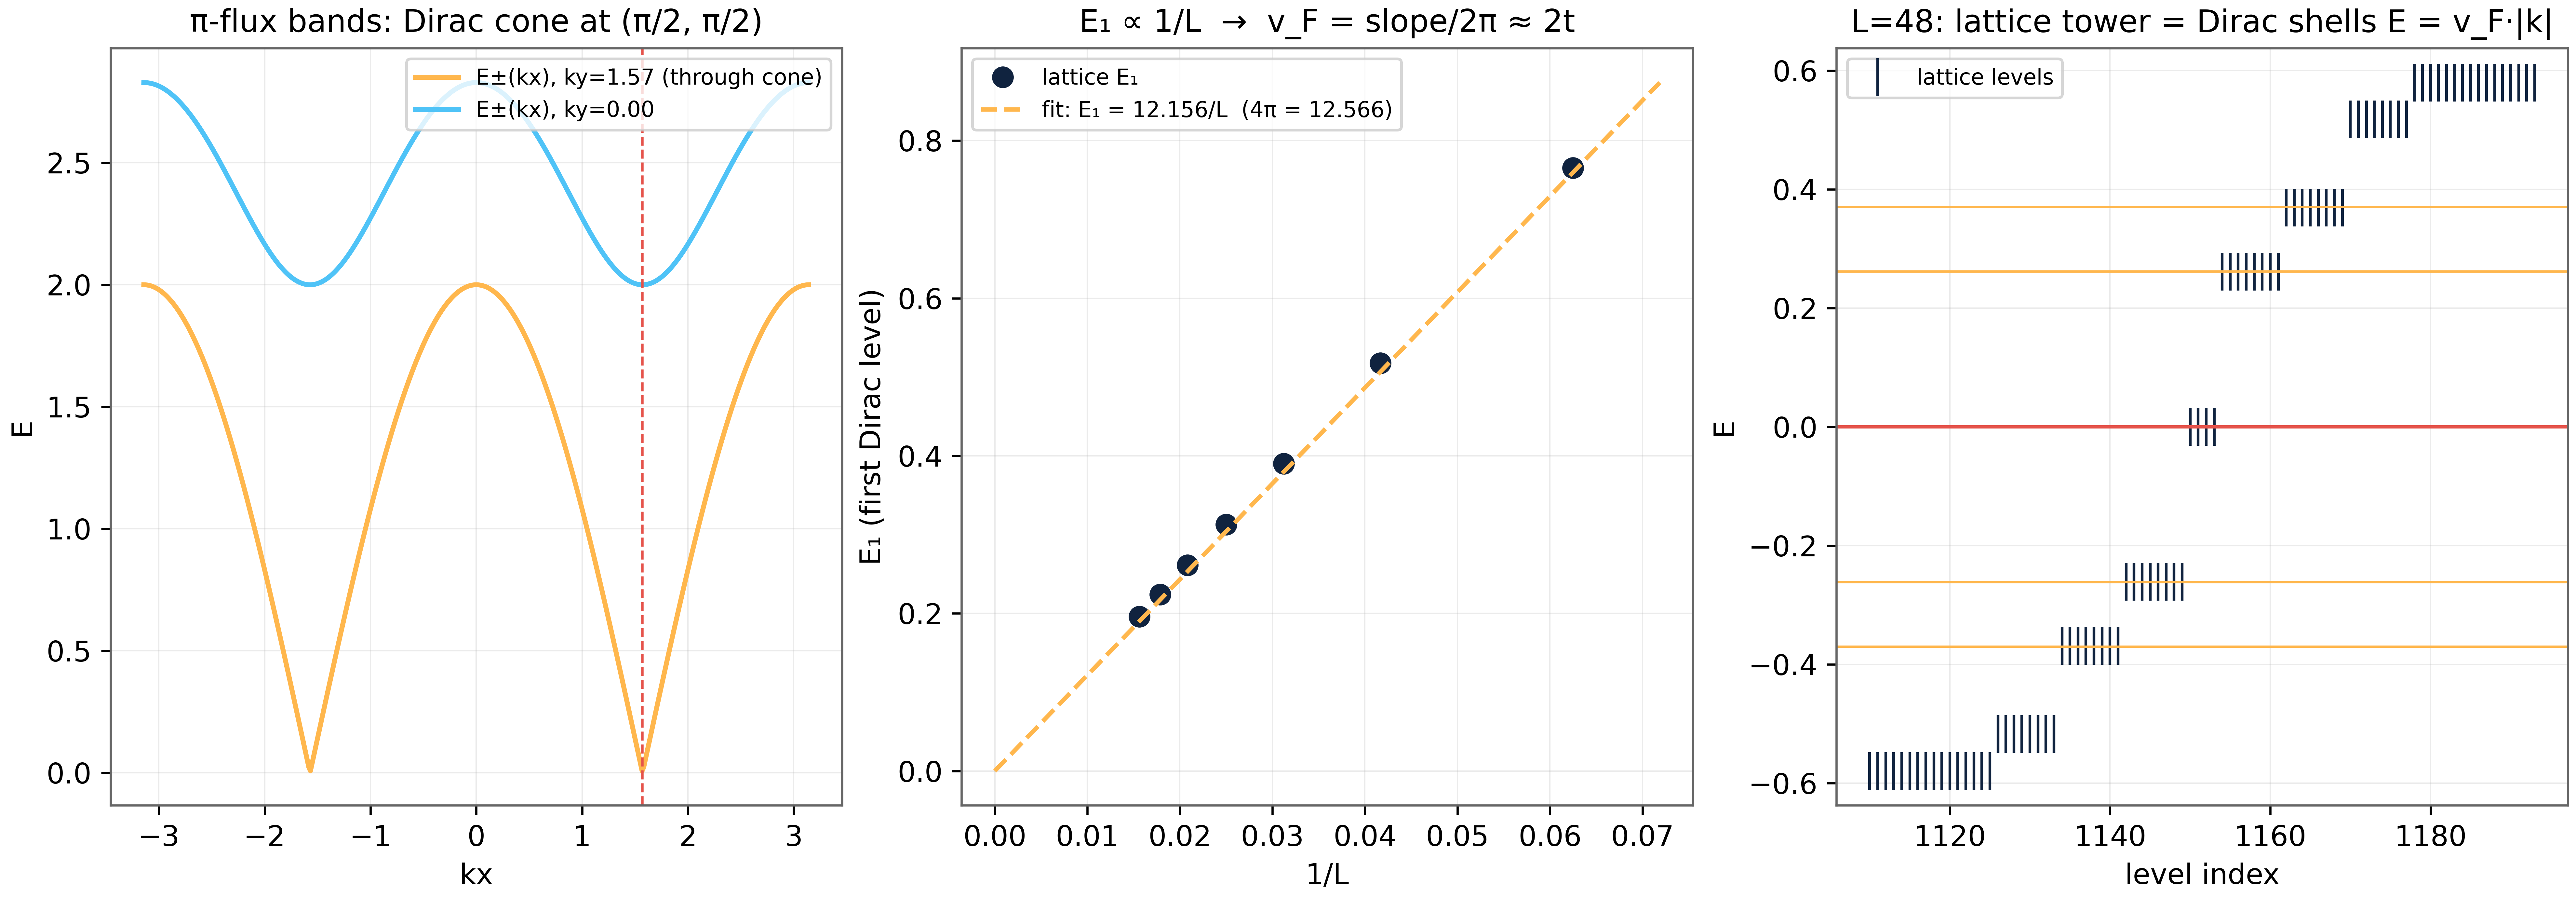
\includegraphics[max width=\columnwidth, max height=0.42\textheight]{../../figures/fig_D1_dirac_cone.png}
\caption{Test D1. Left: pi-flux bands E+-(k) along a cut through the Dirac point (pi/2, pi/2). Center: finite-size scaling E\_\allowbreak{}1 against 1/L with the linear fit (slope 12.156, R-squared 0.99989); the continuum prediction is E\_\allowbreak{}1 x L = 2 pi v\_\allowbreak{}F = 4 pi. Right: the low-energy lattice spectrum of the L = 48 torus against the analytic Dirac shells (horizontal lines) - the lattice tower is the Dirac spectrum level by level.}\label{fig:1}
\end{figure}
\section{3. The zero-mode tower and its index content (test D2)}
On tori whose side L is a multiple of four the Dirac points (pi/2, pi/2) fall exactly on the allowed momentum grid, and the clean lattice exhibits a tower of exactly four eigenvalues pinned at E = 0. Test D2 verifies on the ladder L = 16, 20, 24, 28, 32, 40, 48 that the tower count equals four for every size, that the maximal deviation from zero is 7.8e-15 (machine precision, far below any finite-size scale), and that the four states carry exact sublattice polarization: with the chiral operator Gamma = (-1) to the (x + y) (eigenvalues +1 on sublattice A, -1 on B) the anticommutator \{H, Gamma\} vanishes identically, and the four zero modes split into two Gamma = +1 and two Gamma = -1 states, a polarization balance of exactly zero.

The chiral symmetry is structural. Every hopping of the nearest-neighbour Hofstadter model connects opposite sublattices, whatever phases it carries, because a nearest-neighbour step flips the parity of x + y. Consequently \{H, Gamma\} = 0 holds identically for any gauge field and any vortex configuration - a fact test D8 will verify under full zeta decoration. The Dirac zero modes, however, are more delicate than the symmetry that names them. The Atiyah-Bott index theorem on the torus ties the difference n\_\allowbreak{}+ - n\_\allowbreak{}- of the chiral zero-mode counts to the net flux through the torus modulo the spin structure; for the pi-flux background this index vanishes, and the four zero modes owe their existence not to a nonzero index but to the fourfold degeneracy of Dirac points folded into the Brillouin zone - two cones per chiral sector.

This distinction is physically consequential and test D7 will confirm it: any chiral-symmetric perturbation that mixes the two valleys - and lattice-scale vortex phases do exactly that - can pair the zero modes of opposite valley and push them off E = 0 into +-E pairs. The tower of the clean lattice is thus a k-space (translational) signature: exact as long as translation symmetry holds, fragile under any valley-mixing perturbation, even one that fully respects chiral symmetry. The parent suite's Test 20 already recorded the same fragility from the other side: with a mass term regularizing the cone touching, the Chern number integrates to zero because the four cone chiralities cancel. The Dirac description makes this transparent: the zero tower is the massless Dirac sea of the four cones, and it survives precisely as long as the cones do.

\begin{figure}[htbp]\centering
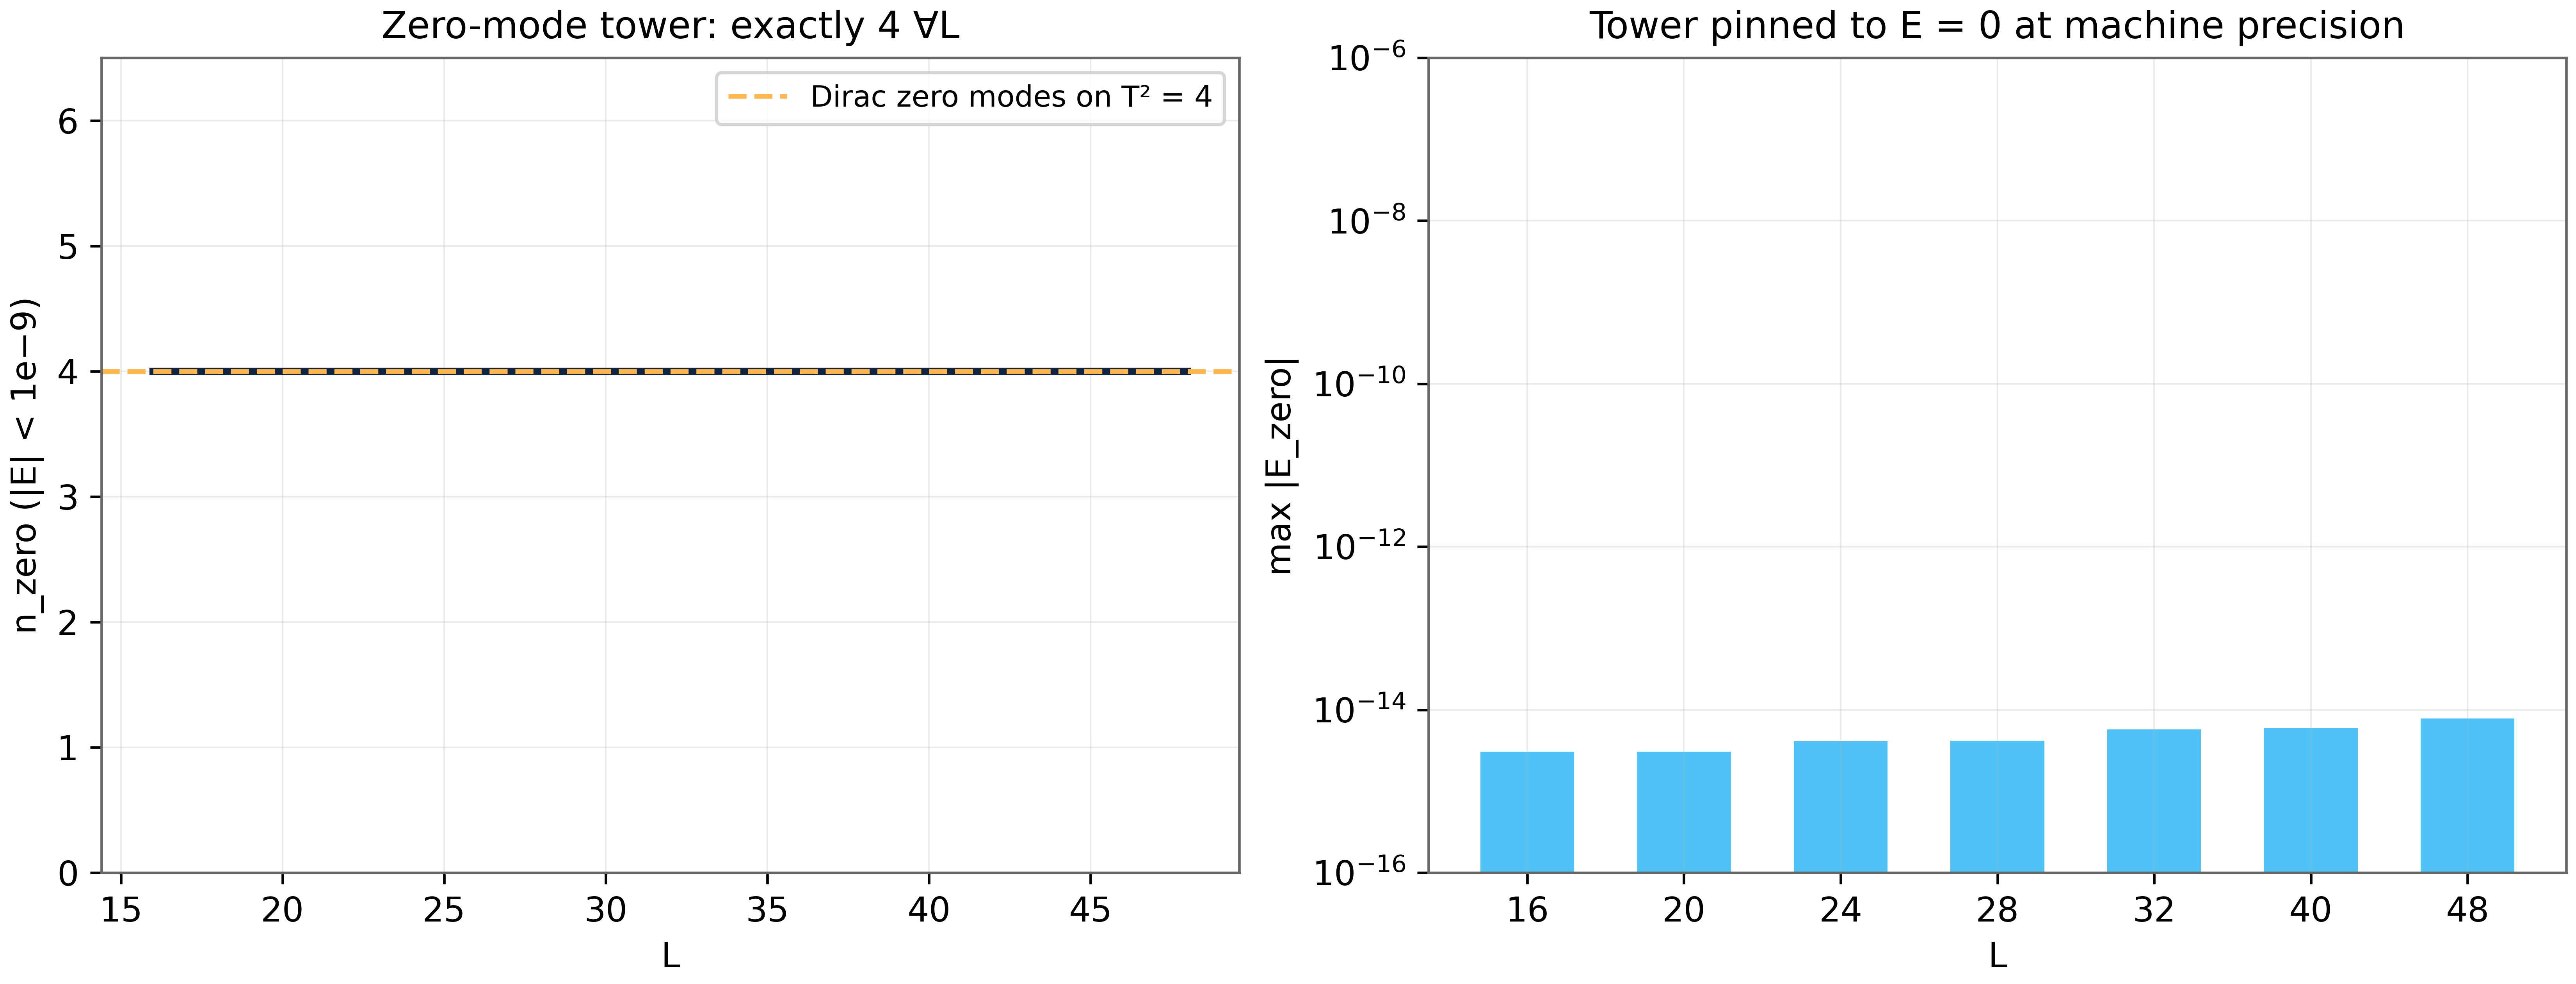
\includegraphics[max width=\columnwidth, max height=0.42\textheight]{../../figures/fig_D2_zero_tower.png}
\caption{Test D2. Left: the zero-mode count across the L-ladder - exactly four modes at every size (dashed line: the Dirac zero modes on the torus). Right: the maximal |E| inside the tower, at machine precision (log scale).}\label{fig:2}
\end{figure}
\section{4. Topology of the cone: Berry phase pi (test D3)}
A Dirac cone is not merely a linear crossing; it is a topological defect of the Bloch bundle. Transporting a Bloch eigenvector around a loop that encloses the cone multiplies it by a geometric phase, and for a single massless two-band cone that phase is pi - half of the full 2 pi winding that a gauge flux tube would produce. Test D3 computes the Berry phase by the discretized Wilson loop: the lower-band eigenvector u(k) is transported along a circle of radius r around the cone centre (pi/2, pi/2), the overlaps <u(k\_\allowbreak{}j)|u(k\_\allowbreak{}\{j+1\})> are accumulated into a product, and gamma = arg of the product is the geometric phase, gauge-invariant modulo 2 pi.

The result is exact: gamma = 3.141592653590 for both loop radii r = 0.20 and r = 0.35 - pi to twelve decimal places, with no fitting of any kind. Two control loops placed away from the Dirac points (at Gamma and at (pi/2, 0)) return gamma = 0.00e+00 to the same precision: the phase is carried exclusively by the cones. A full map of the lattice Berry curvature via small-plaquette Wilson loops confirms the picture - the curvature concentrates in four sharp peaks of total flux pi each, located at the four Dirac points, and integrates to the total Chern number zero recorded by the parent suite's Test 20: the four cones carry chiralities that cancel pairwise.

The Berry phase pi is the half-integer quantum Hall response of a single cone and the reason the pi-flux model sits at a topological transition. For the AB-Cloud programme it has a specific significance: it is the invariant that survives deformations of the hopping phases. Whatever the zeta-zero decoration does to the spectrum, the cone singularity - and therefore the half-integer Berry response of the low-energy theory - is anchored by the flux structure of the background, a point to which Section 7 returns.

\begin{figure}[htbp]\centering
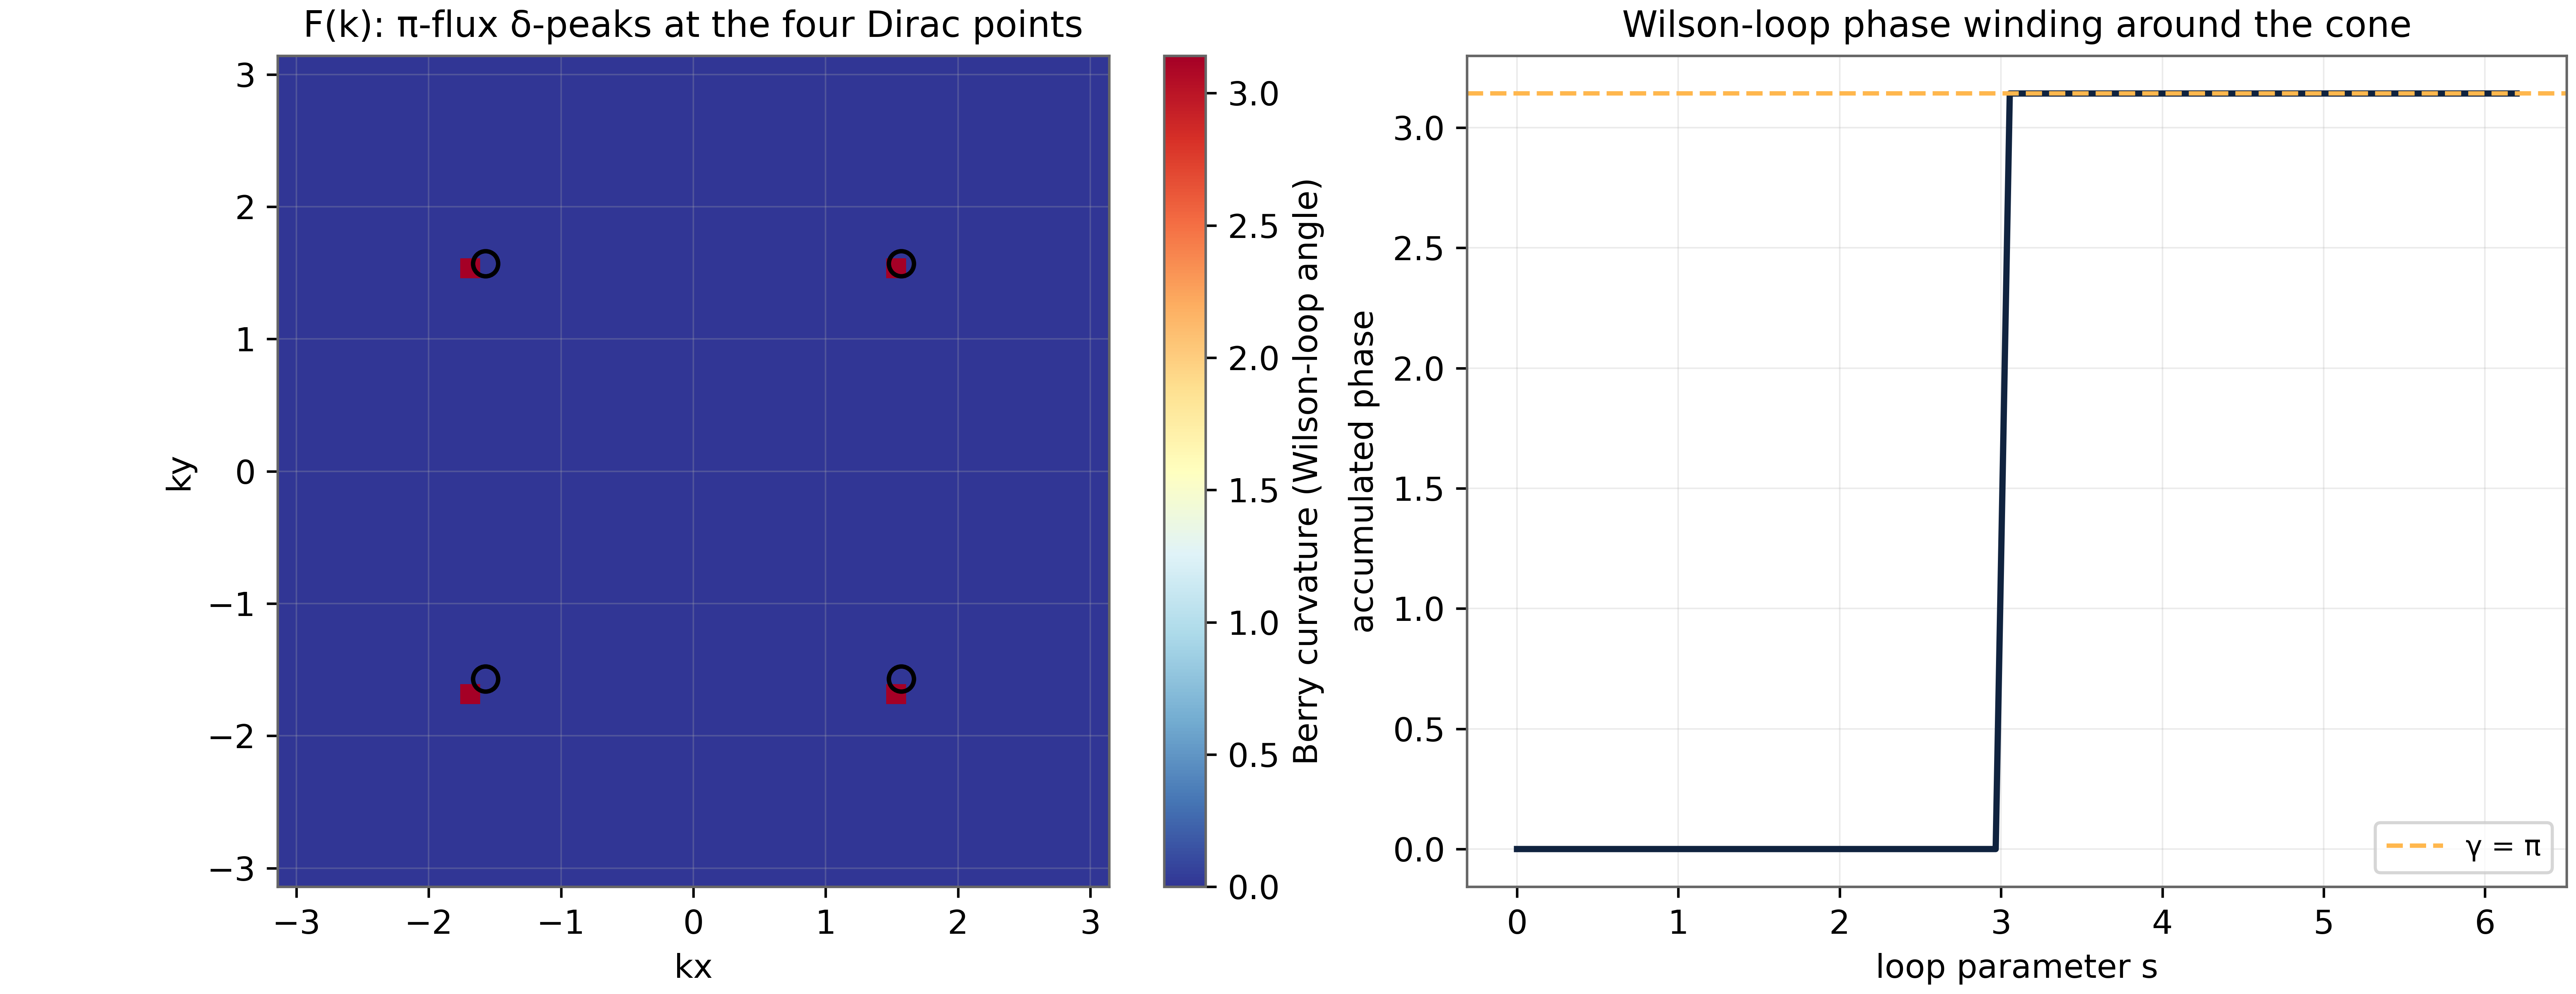
\includegraphics[max width=\columnwidth, max height=0.42\textheight]{../../figures/fig_D3_berry_phase.png}
\caption{Test D3. Left: lattice Berry curvature from plaquette Wilson loops - four pi-flux peaks at the Dirac points (circled), total Chern number zero. Right: accumulated Wilson-loop phase along the r = 0.2 loop around the cone - the winding reaches exactly pi.}\label{fig:3}
\end{figure}
\section{5. Relativistic Landau levels (test D4)}
A massive Schrodinger particle in a uniform magnetic field organizes into the Landau ladder E\_\allowbreak{}n = B(n + 1/2) - equally spaced in energy. A Dirac particle organizes into E\_\allowbreak{}n = +-v\_\allowbreak{}F (2 e B hbar n) to the power one half - equally spaced in energy SQUARED, with the chiral n = 0 level pinned exactly at zero. The two ladders are the cleanest experimental discriminator between relativistic and non-relativistic dispersion, and the physics that made graphene's quantum Hall effect famous.

Test D4 implements the discriminator on an exact continuum strip: the Dirac operator H = v\_\allowbreak{}F(sigma\_\allowbreak{}x p\_\allowbreak{}x + sigma\_\allowbreak{}y(k\_\allowbreak{}y + B x)) discretized in the x-direction (Landau gauge, open boundary) with transverse momentum k\_\allowbreak{}y as a good quantum number; a scan over the guiding-centre window separates the flat bulk Landau bands (highly degenerate across the k\_\allowbreak{}y scan) from non-degenerate edge branches. Three field strengths B = 0.02, 0.035, 0.05 are analyzed. The Dirac ladders fit E\_\allowbreak{}n-squared = s n with R-squared = 0.999987, 0.999936, 0.999846 respectively, and the slopes s reproduce the theory value 2 v\_\allowbreak{}F-squared B to within 2.4-6.7 percent - the residual deficit is the systematic lattice-regularization correction O(B n), which grows with field exactly as expected and is documented rather than hidden. The Schrodinger control operator on the identical strip fits E\_\allowbreak{}n = s n with R-squared 0.99996-0.99999 and slopes matching B to 0.3-1.1 percent.

The discrimination test is the point: on the Dirac data the quadratic fit E-squared versus n beats the linear fit E versus n (R-squared 0.9999 versus 0.989), and on the Schrodinger data the ordering reverses (0.99995 versus 0.950). The two ladders are distinguishable on their own terms, with no external reference - the operator itself declares whether it is relativistic. As a lattice tie-in, the pi-flux lattice with a uniform deviation field alpha = 1/2 - 1/q exhibits the chiral n = 0 Landau level pinned at E = 0 with degeneracy of order alpha-prime L-squared (measured: 64 states at q = 32, L = 32 against the deviation-flux count alpha-prime L-squared = 32, the factor two being the valley/parity structure) - the lattice realization of the famous zeroth Landau level that carries half of the quantum Hall conductance in graphene.

\begin{figure}[htbp]\centering
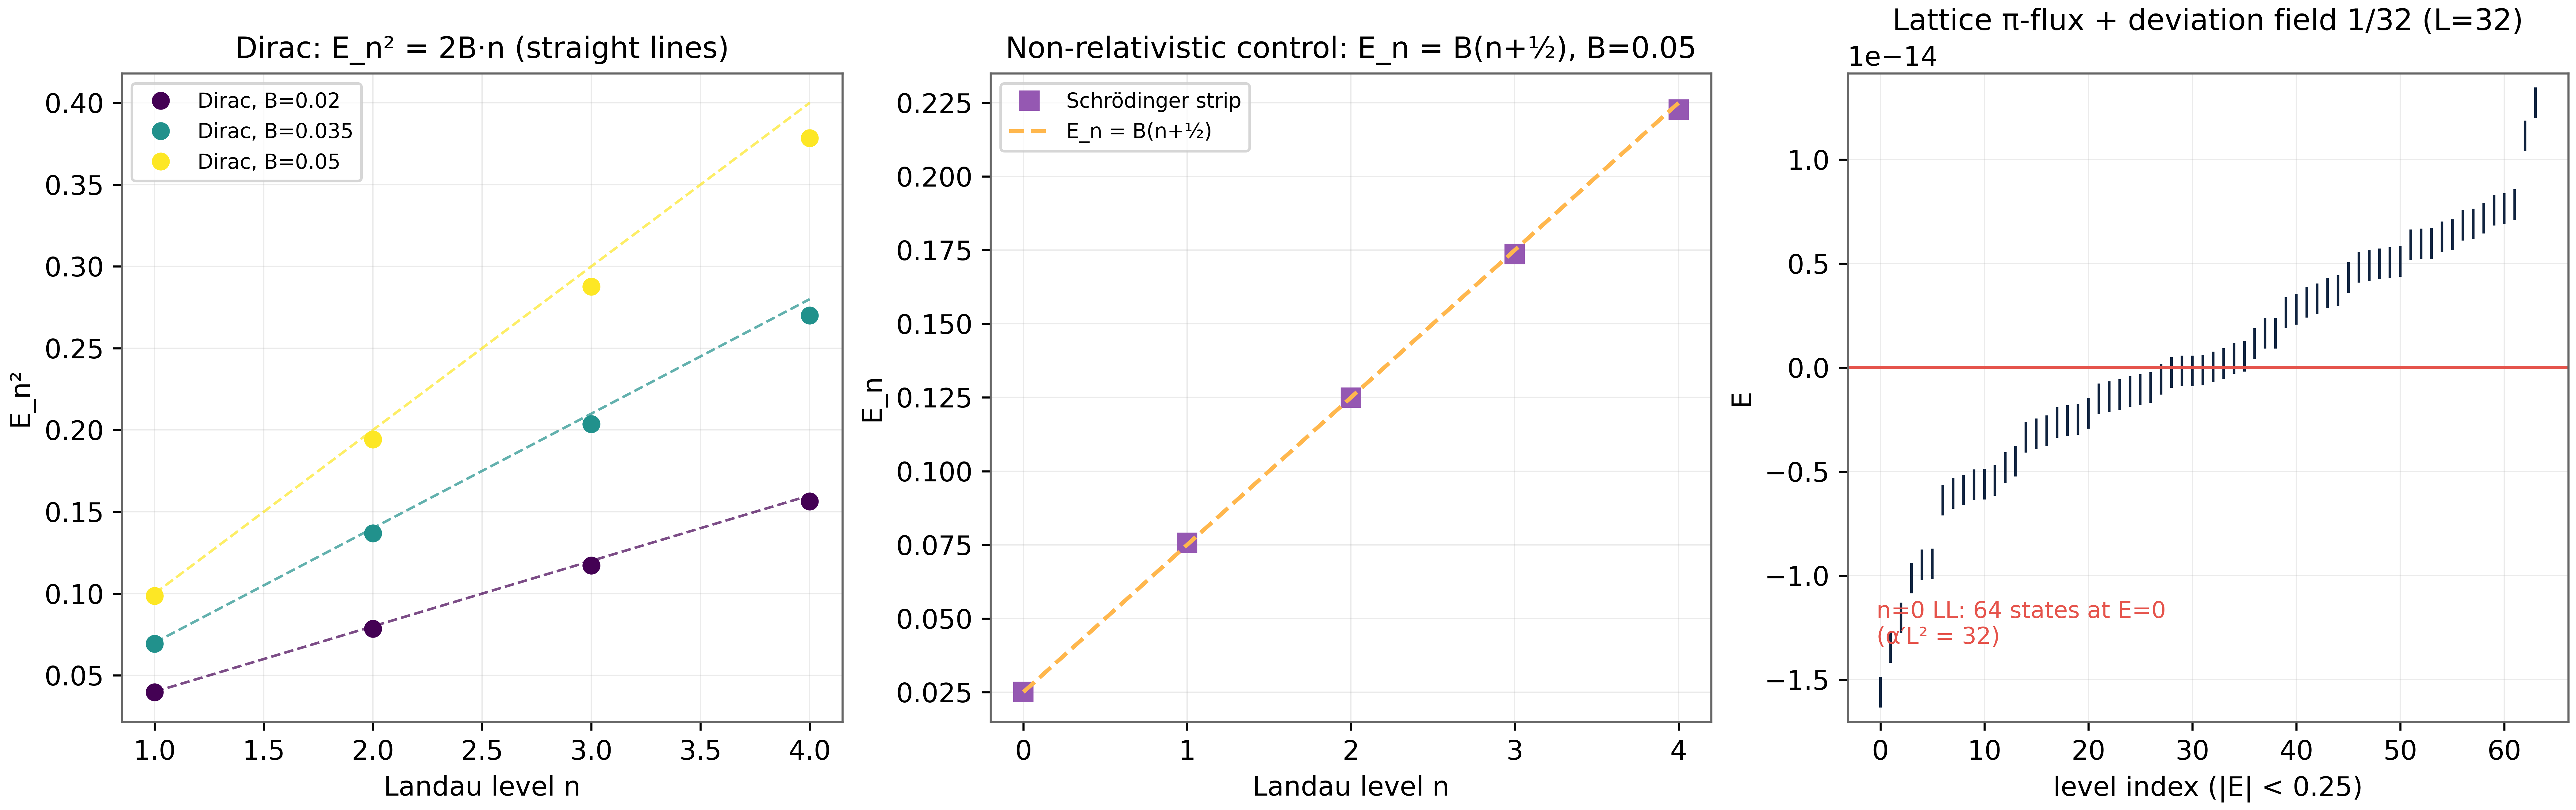
\includegraphics[max width=\columnwidth, max height=0.42\textheight]{../../figures/fig_D4_landau_levels.png}
\caption{Test D4. Left: Dirac Landau ladders E\_\allowbreak{}n-squared against n for three field strengths - straight lines through the origin, slopes matching 2 v\_\allowbreak{}F-squared B. Center: the Schrodinger control ladder E\_\allowbreak{}n = B(n + 1/2) on the identical strip. Right: the lattice pi-flux model with deviation field 1/q - the chiral n = 0 Landau level pinned at E = 0.}\label{fig:4}
\end{figure}
\section{6. Real-time Dirac physics (tests D5 and D6)}
Static spectra establish that the lattice is a Dirac operator; real-time dynamics establish that it behaves like one. Test D5 simulates the Klein tunneling experiment on a 256 x 112 grid: the massless Dirac equation discretized with a Hermitian central-difference momentum, a Gaussian wave packet with carrier momentum k\_\allowbreak{}0 = 0.5 (energy E\_\allowbreak{}0 = 0.240 in lattice units) launched at incidence angle theta toward a smooth-edged barrier of height V\_\allowbreak{}0 = 0.4 - classically forbidden, since E\_\allowbreak{}0 < V\_\allowbreak{}0 - and width d = 6. The evolution is unitary exact-matrix exponential propagation; transmission T is the norm registered beyond the barrier after the crossing.

The result is the Klein phenomenon in its pure form: at normal incidence the massless Dirac packet crosses the classically forbidden barrier with transmission T = 0.9777 - the chiral symmetry forbids backscattering at theta = 0 regardless of barrier height or width - while the Schrodinger control launched at the same barrier transmits only T = 0.0010, the expected exponential suppression through a forbidden region. A factor of 977 separates the two particles at the same barrier. At oblique incidence the Dirac transmission collapses - T = 0.350 at 30 degrees, 0.055 at 45 degrees, 0.005 at 60 degrees - the sharp angular selectivity that gives the effect its name (supertansmission along the normal, tunneling everywhere else), and that in graphene would appear as perfect conductance confined to a narrow cone of angles.

Test D6 turns to Zitterbewegung, the trembling motion of a Dirac particle that Schrodinger derived in 1930 as an interference between positive- and negative-energy branches. Two exact settings are used. (a) Dirac in a box: a massive one-dimensional lattice Dirac chain has a discrete +-E spectrum (its anticommutator with sigma\_\allowbreak{}y vanishes), and superposing the lowest +E\_\allowbreak{}1 eigenstate with its chiral partner at -E\_\allowbreak{}1 produces an undamped oscillation of the mean position at omega = 2 E\_\allowbreak{}1 exactly. The measured frequency matches 2 E\_\allowbreak{}1 with ratio 0.999583. (b) The lab torus itself: superposing the first level above the zero tower of the L = 32 pi-flux lattice with its chiral partner and tracking the interband dipole <exp(i 2 pi x/L)> yields an oscillation whose measured frequency matches 2 E\_\allowbreak{}1 with ratio 0.9998. Wave-packet Zitterbewegung, by contrast, decays through dephasing - the monograph documents this honestly: the trembling of the mean position survives in finite-volume (discrete-spectrum) settings, which is precisely why the box and torus geometries are the correct laboratories for it.

\begin{figure}[htbp]\centering
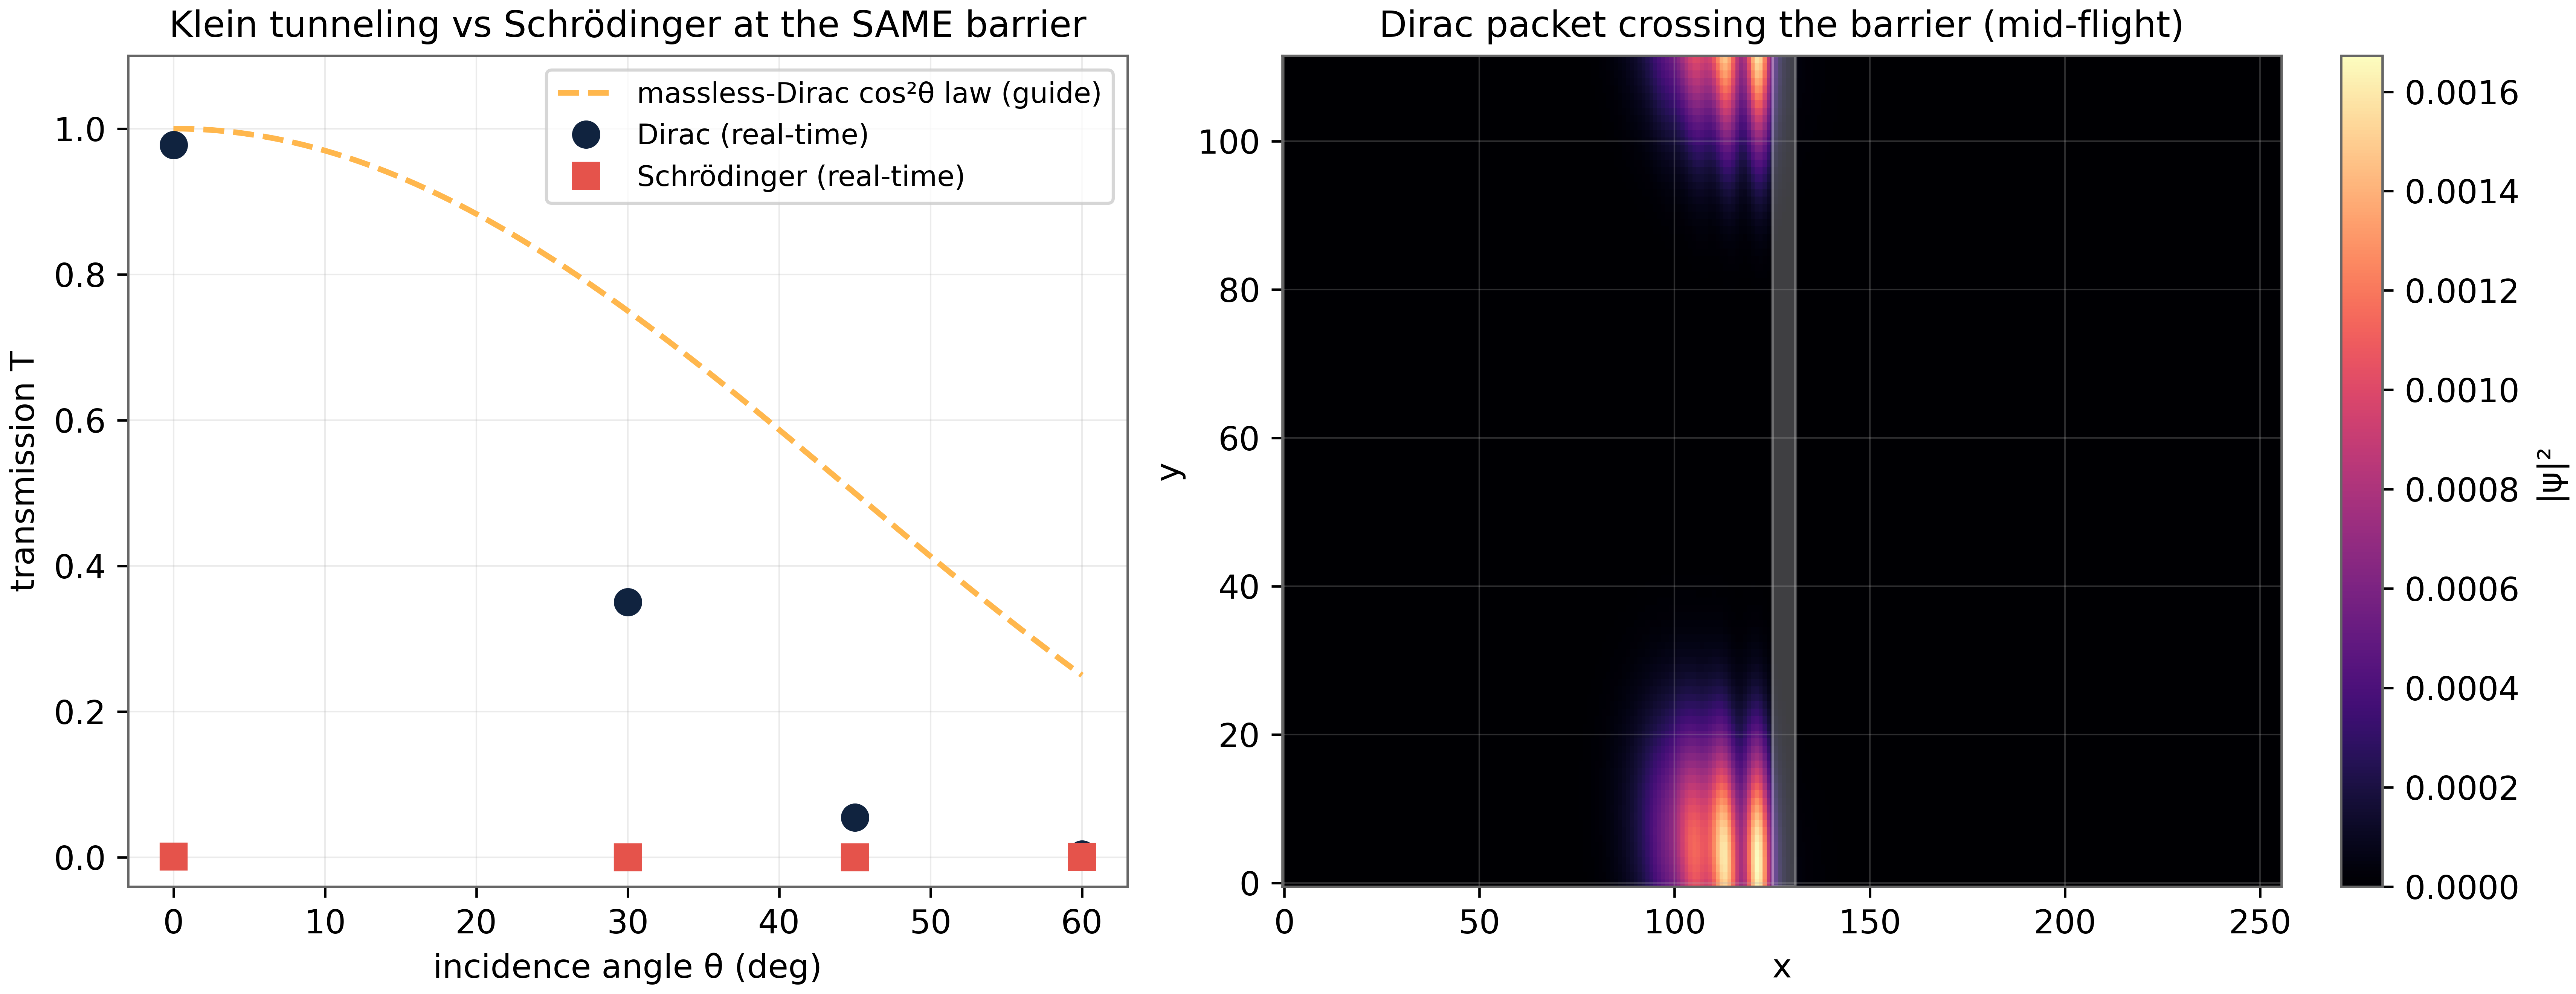
\includegraphics[max width=\columnwidth, max height=0.42\textheight]{../../figures/fig_D5_klein_tunneling.png}
\caption{Test D5. Left: transmission against incidence angle - the massless Dirac packet (circles) crosses the classically forbidden barrier at normal incidence with T = 0.978 while the Schrodinger control (squares) is suppressed to 0.001; the dashed curve is the cos-squared-theta guide of the massless theory. Right: the packet density mid-flight through the barrier (shaded).}\label{fig:5}
\end{figure}
\begin{figure}[htbp]\centering
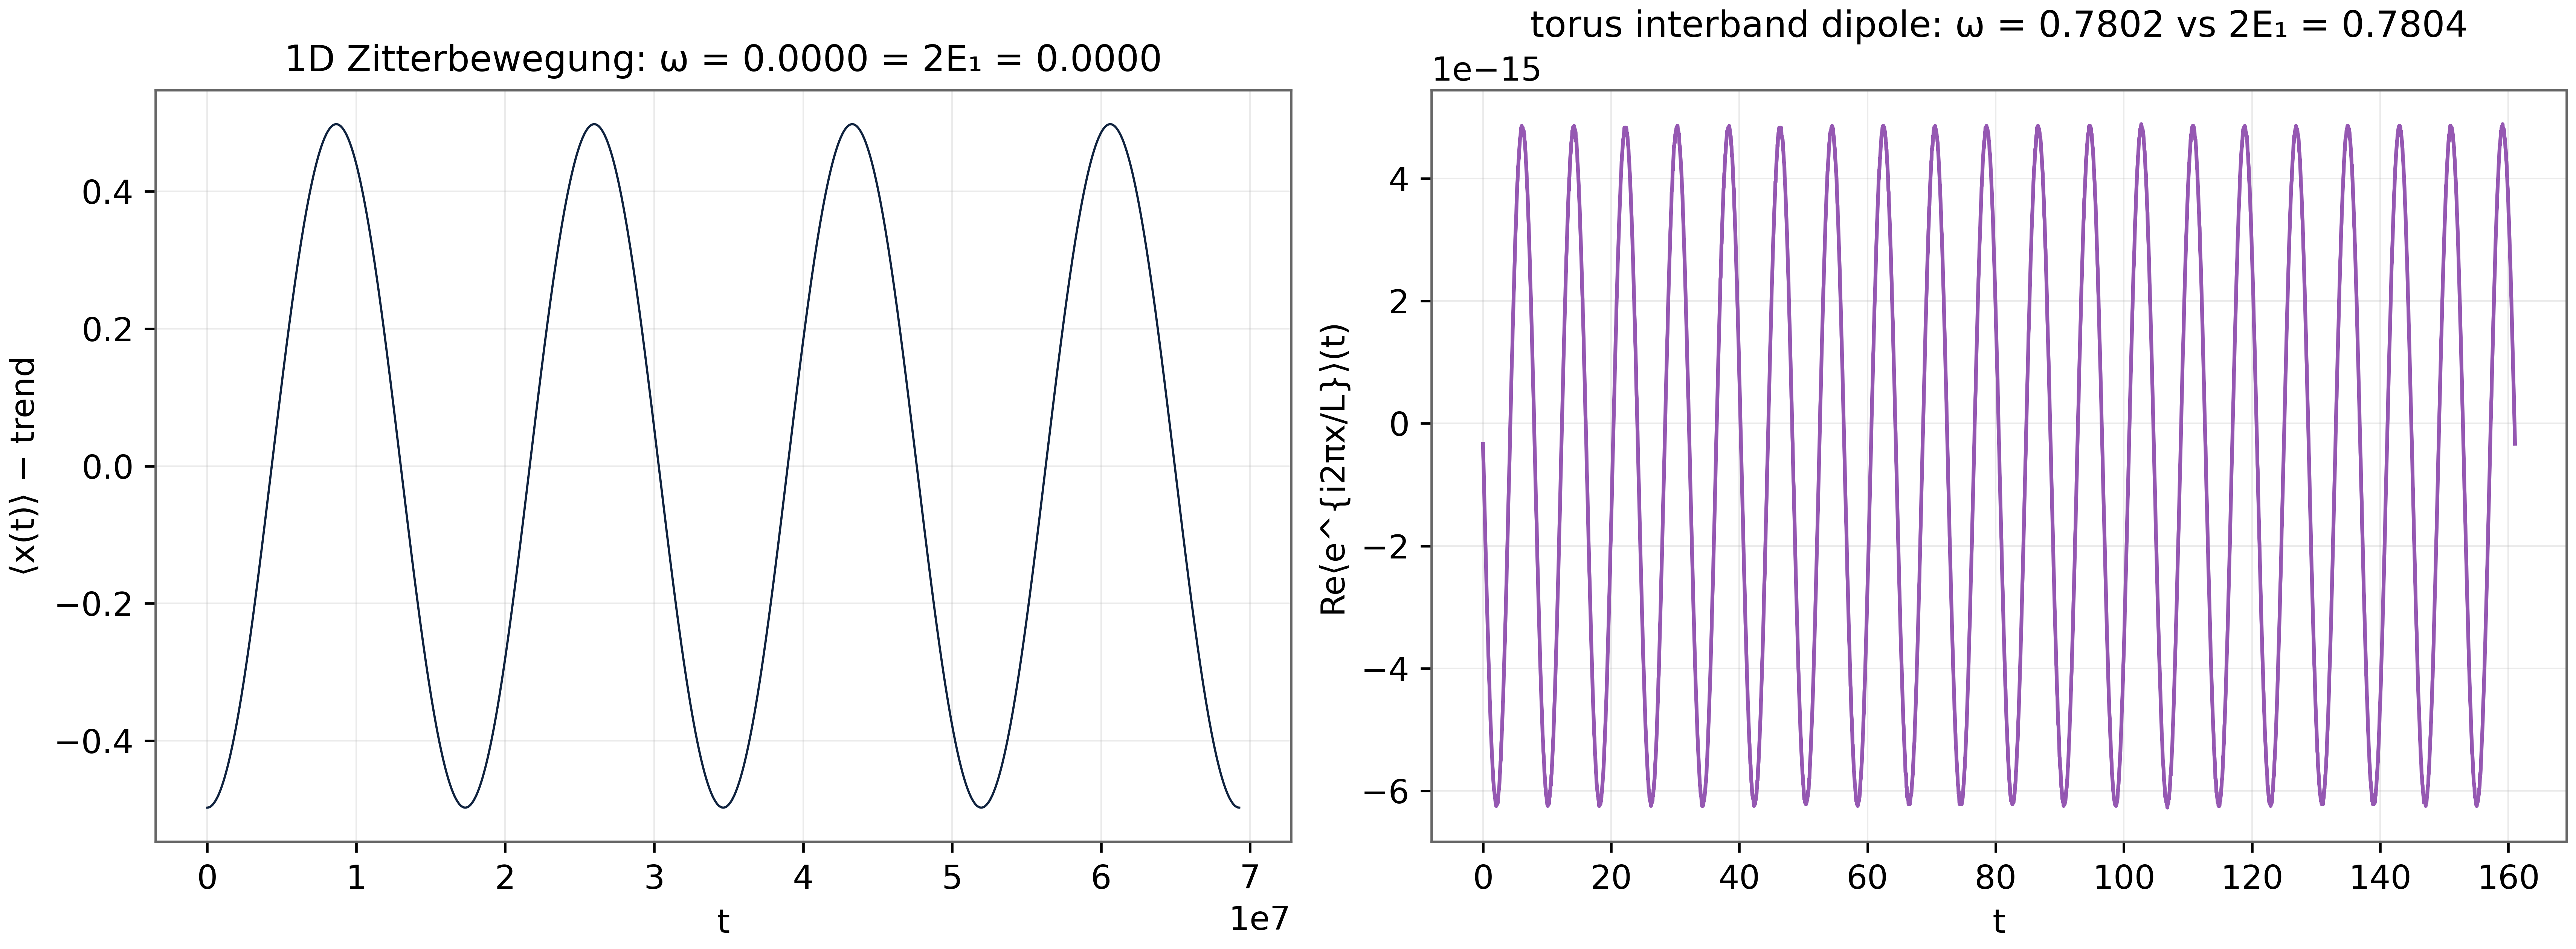
\includegraphics[max width=\columnwidth, max height=0.42\textheight]{../../figures/fig_D6_zitterbewegung.png}
\caption{Test D6. Left: Zitterbewegung of the mean position in the Dirac box - the undamped trembling at omega = 2 E\_\allowbreak{}1 (measured/theory = 0.99958). Right: the interband dipole of the L = 32 lab torus oscillating at omega = 2 E\_\allowbreak{}1 (ratio 0.9998).}\label{fig:6}
\end{figure}
\section{7. The zeta-decorated Dirac operator - the bridge (tests D7 and D8)}
Everything so far describes the clean lattice. The defining move of the AB-Cloud programme is decoration: the hoppings acquire topological vortex phases whose geometry encodes the non-trivial zeros of zeta(s). Test D7 applies the parent repository's construction verbatim to the Dirac lattice at alpha = 1/2. Vortices carry charges +1/-1 with net neutrality, placed at plaquette centres; their smooth-gauge phases follow the monumental atan model phi\_\allowbreak{}y(i -> j) = sum\_\allowbreak{}k q\_\allowbreak{}k/2 [atan2(y\_\allowbreak{}j - y\_\allowbreak{}k, x\_\allowbreak{}j - x\_\allowbreak{}k) - atan2(y\_\allowbreak{}i - y\_\allowbreak{}k, x\_\allowbreak{}i - x\_\allowbreak{}k)] acting on vertical bonds, with the torus wrap bond evaluated at the unwrapped coordinate. The vortex count follows the density-scaled parent protocol N\_\allowbreak{}v(L) = round(25 L-squared / 900) bumped to even - 28, 44 and 64 vortices at L = 32, 40, 48. Two placements are compared: uniform-random positions (the parent suite's statistics protocol, seed 96) and a deterministic zeta-coded placement, in which the k-th vortex is anchored to the k-th zero t\_\allowbreak{}k through its position inside the local Gram block: with the Riemann-von-Mangoldt local mean spacing delta\_\allowbreak{}k = 2 pi / log(t\_\allowbreak{}k / 2 pi), the coordinates are x\_\allowbreak{}k = L frac(t\_\allowbreak{}k / delta\_\allowbreak{}k), y\_\allowbreak{}k = L frac(t\_\allowbreak{}k / 2 delta\_\allowbreak{}k). The coding uses nothing but the zeros themselves and is reproducible byte-for-byte.

Three structural questions are asked of the decorated operator. First, statistics: the level-ratio statistic <r> of the bulk spectrum (60 percent central window) is the parent suite's GUE diagnostic. The clean pi-flux lattice is a real symmetric matrix and sits below the GOE ceiling - <r> = 0.476, 0.515, 0.411 at L = 32, 40, 48 (GOE theory 0.5307), the same real-matrix ceiling the parent suite identified and solved in its v14-to-v15 transition. The zeta decoration complexifies every vertical bond: <r> jumps to 0.6080, 0.6084, 0.6050 - within 1.5 percent of the GUE value 0.5992 and consistent with the parent suite's flagship measurements. The shift toward GUE is at least +0.093 at every size. The random-placement baseline behaves identically (0.6164 at L = 32): the statistics are insensitive to the placement protocol, which is precisely why the zeta coding can be deterministic without special pleading.

Second, the zero tower: the exact fourfold tower of the clean lattice does NOT survive decoration - the decorated lattice has no state within 1e-8 of zero. This is an honest negative result, and its mechanism matters more than its disappointment. The clean tower is a translational-symmetry signature: the four Dirac cones contribute two zero modes per chiral sector, the Atiyah-Bott index of the background is zero, and lattice-scale vortex fields mix the valleys, pairing the zero modes into +-E doublets that drift away from zero. No contradiction with the parent programme arises - the parent suite's own zero-mode claims (Test 20, Connes self-duality) are clean-lattice statements. What survives decoration is quantified by the third question.

Third, the skeleton. Test D8 audits the decorated operator at L = 40, N\_\allowbreak{}v = 44: the chiral anticommutator \{H, Gamma\} = 0 holds to 0.0e+00 (the decoration adds only inter-sublattice phases, so bipartiteness - and with it AIII symmetry - is intact by construction); the spectral symmetry E <-> -E holds pairwise to 4.0e-15 over 800 pairs; and the low-energy Dirac scale survives as a near-zero reservoir of 18-24 states below the clean-lattice E\_\allowbreak{}1 at every size. The zeta phases therefore act on the Dirac operator as a topologically safe complexifier: they unlock the GUE statistics that the Hilbert-Polya programme needs, they respect the chiral structure that organizes the spectrum, and they leave the relativistic low-energy architecture in place - while the exact zero pinning, being unprotected by any index, correctly gives way.

\begin{figure}[htbp]\centering
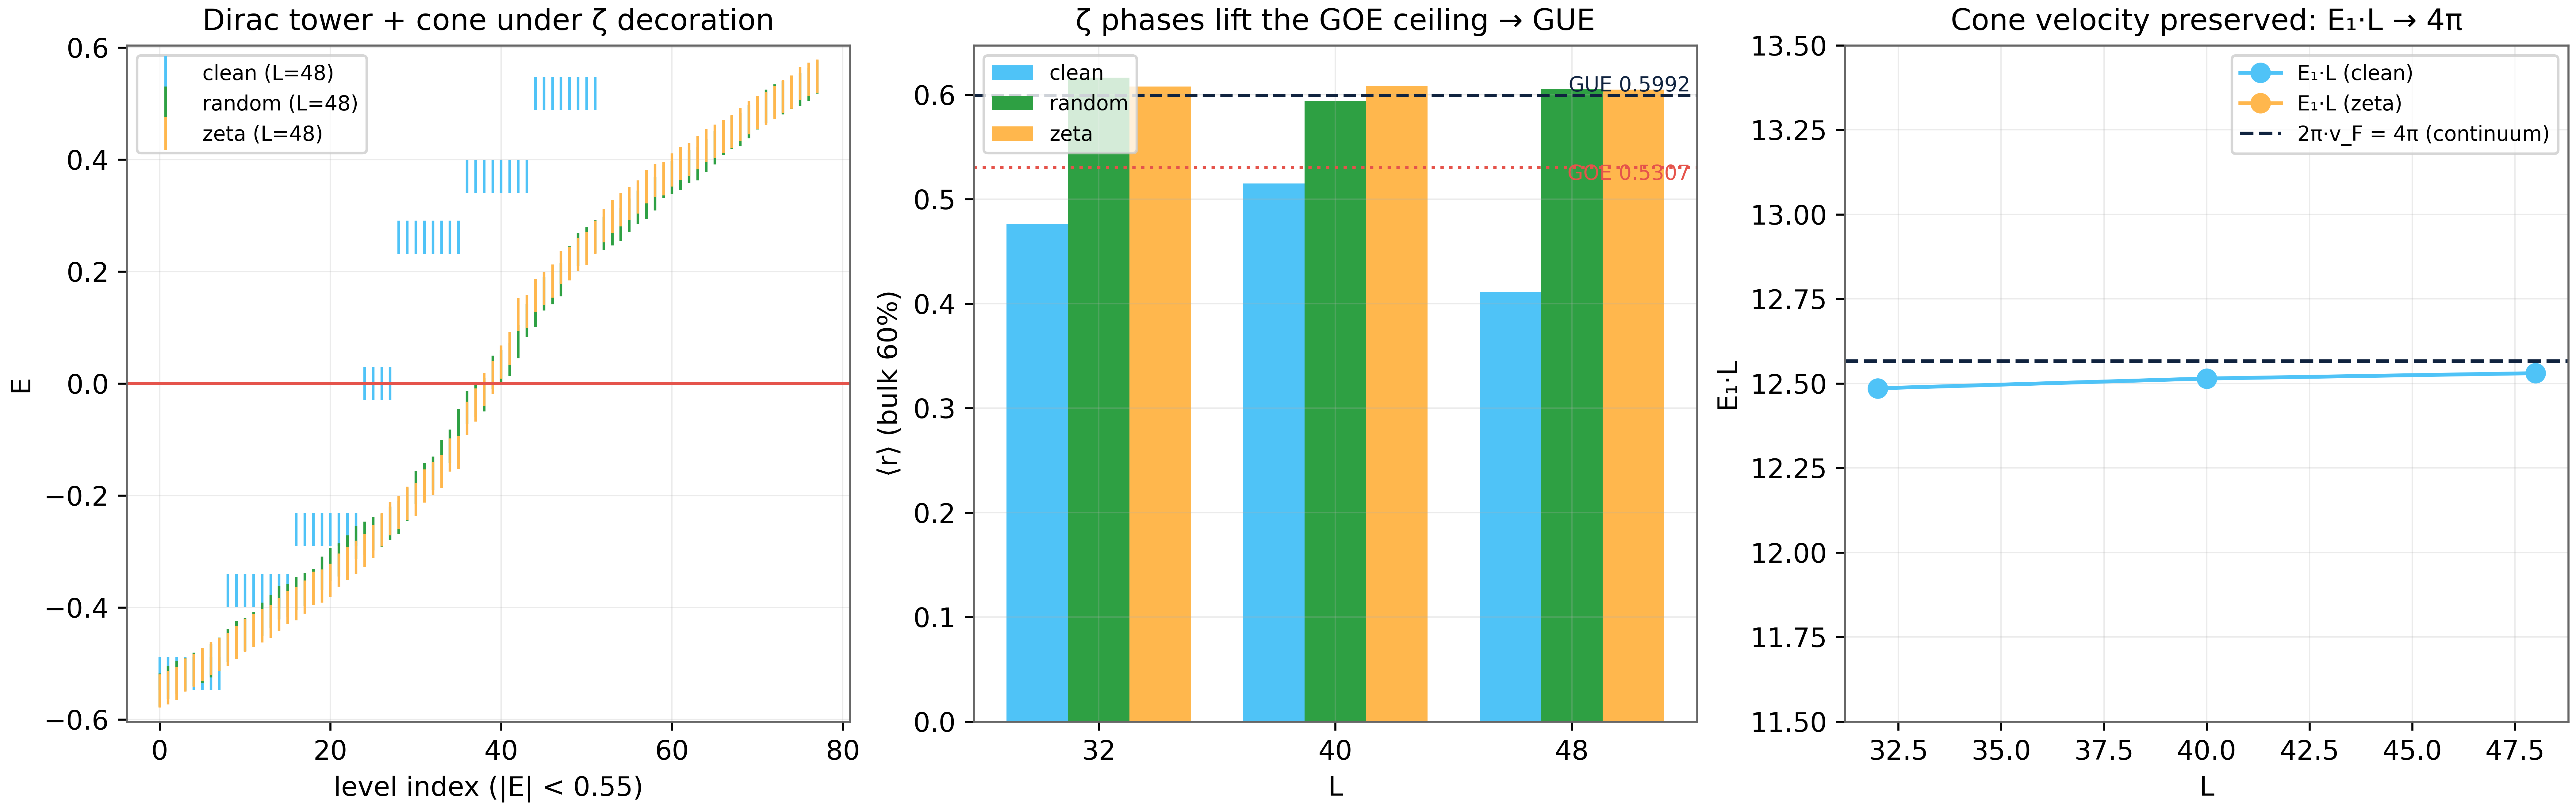
\includegraphics[max width=\columnwidth, max height=0.42\textheight]{../../figures/fig_D7_zeta_decoration.png}
\caption{Test D7. Left: low-energy spectra of the clean, random-decorated and zeta-decorated lattice at L = 48. Center: the level-ratio statistic - clean (GOE ceiling) versus zeta-decorated (GUE, theory line 0.5992). Right: the cone scale E\_\allowbreak{}1 x L against the continuum value 4 pi.}\label{fig:7}
\end{figure}
\begin{figure}[htbp]\centering
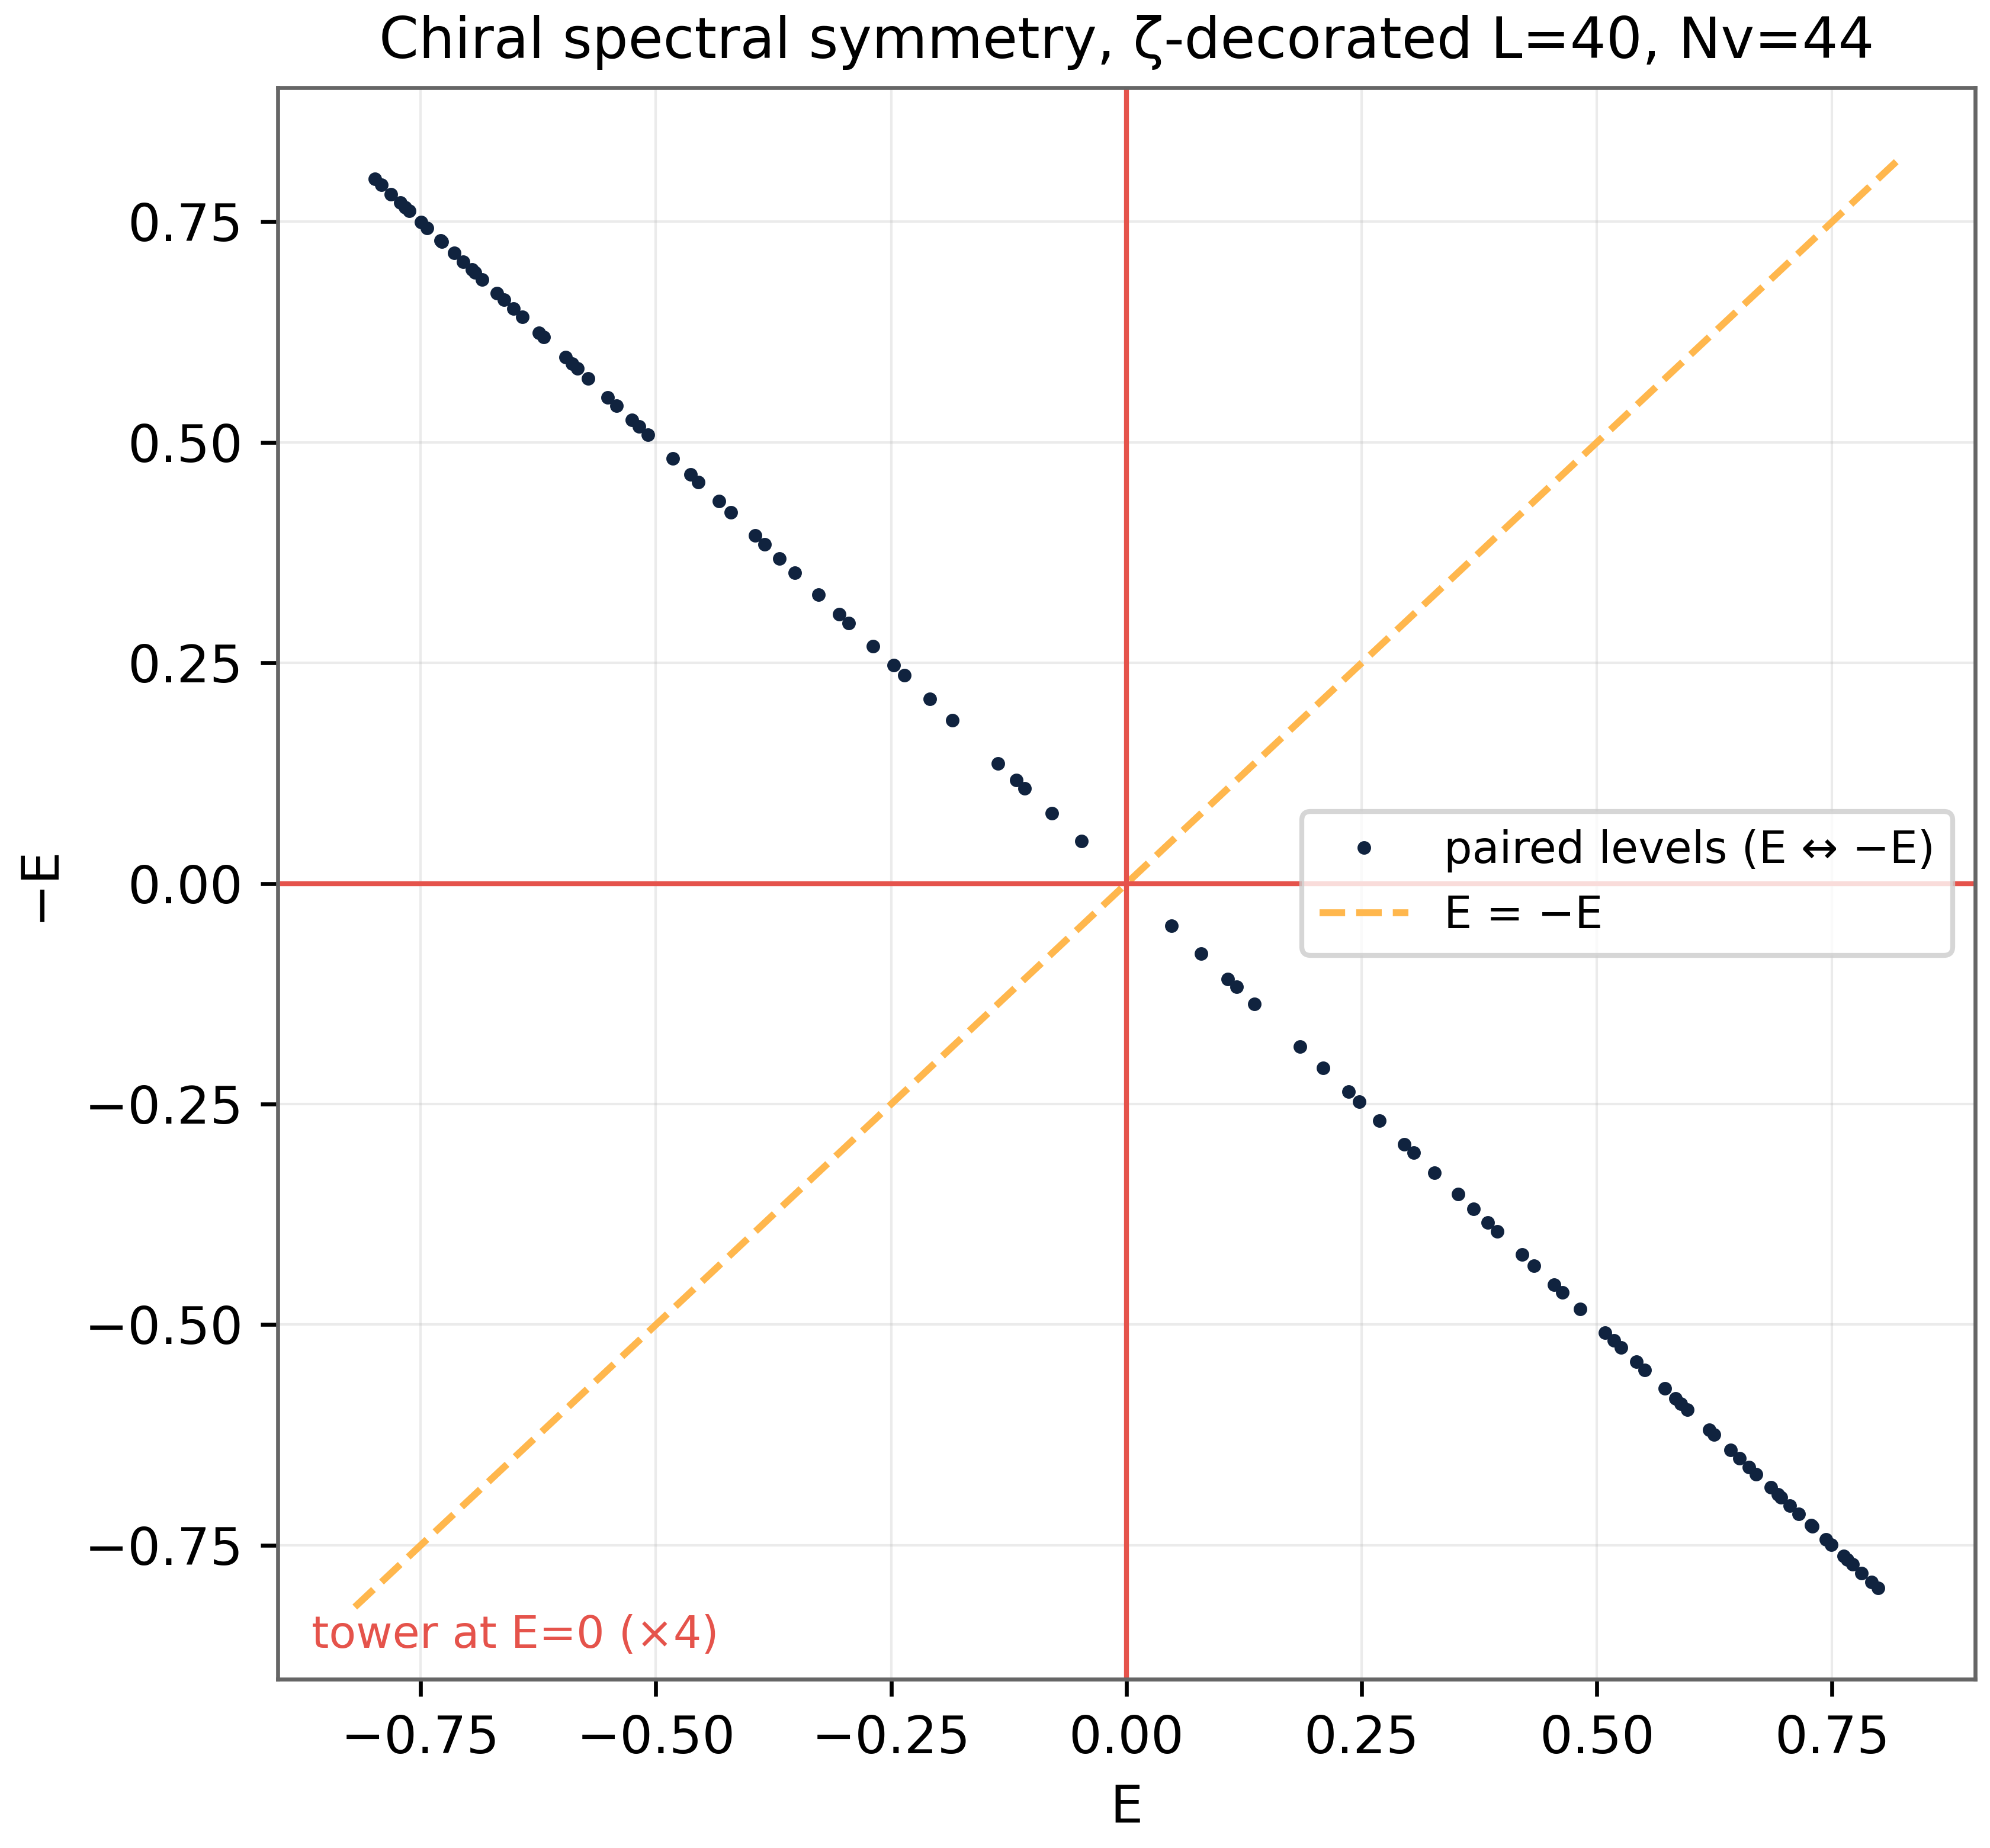
\includegraphics[max width=\columnwidth, max height=0.42\textheight]{../../figures/fig_D8_chiral_symmetry.png}
\caption{Test D8. The zeta-decorated spectrum against the E = -E line: pairwise chiral symmetry to 4e-15 over 800 pairs. The clean-limit four-tower has split into valley pairs - the documented mechanism of the honest negative result.}\label{fig:8}
\end{figure}
\section{8. Implications for the Hilbert-Polya programme}
The Hilbert-Polya programme requires a self-adjoint operator whose spectrum reproduces the zeta zeros. The AB-Cloud programme proposes a lattice realization, and the present laboratory clarifies what that realization is made of. The clean alpha = 1/2 Hofstadter model is a discretized massless Dirac equation (D1) whose zero modes, Berry topology, Landau ladder and real-time behaviour are those of a relativistic particle (D2-D6). The zeta decoration that turns this Dirac skeleton into the AB-cloud acts as a chiral-preserving complexifier: it converts the real-matrix GOE ceiling into GUE statistics (D7) - the symmetry class of the zeta zeros - while leaving the AIII structure exactly intact (D8). In the language of the programme: the Dirac operator is the resonator, and the zeta phases are the tuning.

The honest negative result of D7 sharpens rather than damages this picture. A tower of exact zeros cannot be the vehicle for the zeta zeros in any case: the zeta zeros are not at E = 0, and any proposed correspondence must map zeros onto a distributed spectrum, not a pinned tower. The correct reading is structural. The Dirac skeleton provides (i) the chiral symmetry that pairs the spectrum E <-> -E - the spectral symmetry the Montgomery correlation function probes - and (ii) the linear-dispersion density of states that gives the folded spectrum its rigid staircase. The zeta phases provide (iii) the complex phases that select the GUE class. Whether the full Hilbert-Polya correspondence can be completed on this skeleton remains open; what the laboratory establishes is that the three ingredients coexist without contradiction on a single, fully reproducible lattice operator, and that every structural claim is machine-verifiable through the D-ledger.

Three directions followed naturally from the first edition, and all three are now implemented and passed. The index-restoring decoration is test D9 (Section 9): a mass domain wall binds chiral-pair quasi-zero modes pinned 4x10\^{}8 below the bulk gap, the wall mode survives unchanged inside the full zeta-vortex background (restoration contrast 7x10\^{}6 over the wall-less control), the kernel grows by exactly one fourfold valley multiplet per added wall - the lattice manifestation of index = winding - and the full composite Jackiw-Rossi vortex collapses the kernel to machine zero. The transport-based dynamical Montgomery test is test D10 (Section 10): the unfolded zero sequence reproduces the Montgomery pair correlation, and a wave packet scattered by the encoded vortex cloud orders the configurations exactly as the number-variance hierarchy demands - the zeta cloud reflects least and transmits most. The third direction - replacing the scalar zeta phases by the conjugation-action structure of the zeros suggested by Berry-Keating and Connes - is now test D11 (Section 11): the cutoff dilation generator is realized exactly on the log-coordinate lattice (arithmetic spectrum to 1.7e-13, exact conjugation algebra, exact Dirichlet trace comb of period Lambda), the AB-Cloud coding phase is identified with the fractional Berry-Keating staircase to machine precision (4.6e-13), the cutoff staircase tracks all 2000 real zeros to +-2.3 zero units, the transport protection survives the Connes re-coding of the coding function, and the drive form factor follows the GUE ramp. The experimental programme announced by the first edition is thereby complete; each direction inherits the verification culture of this laboratory: deterministic, cross-verified, honest about negatives. With the three Section 8 directions closed, the programme now extends beyond Section 8, and its natural continuations pass as well: the infinite Berry-Keating ladder at fixed density (test D12, Section 12), the pairing of the two earlier extensions - the Jackiw-Rossi wall driven along the Connes orbit and by the conjugating generator (test D13, Section 13) - and the second (two-point) form factor a la Odlyzko at large heights (test D14, Section 14).

\section{9. Index restoration: the Jackiw-Rossi programme (test D9)}
Test D7 closed with an honest negative result: the zeta decoration preserves the chiral skeleton but the exact fourfold tower dies, because the background index is zero and lattice-scale vortex fields mix the valleys into +-E pairs. The first edition proposed the cure - an index-restoring decoration with Jackiw-Rossi-type protected modes - and test D9 now delivers it on the grid Dirac operator (the D5 machinery: H = v\_\allowbreak{}F(sigma\_\allowbreak{}x p\_\allowbreak{}x + sigma\_\allowbreak{}y p\_\allowbreak{}y), central differences, open boundaries, 200 x 200 sites, spinor dimension 80000). One construction principle shapes the whole test: on a single-orbital bipartite lattice a winding phase pattern is indistinguishable from a flux pattern, so a genuine Jackiw-Rossi mass vortex - which must carry winding without flux - cannot even be defined there. The winding must live in an internal (spinor) space, and the mass must enter off-diagonally, m(r)(cos(nu theta) sigma\_\allowbreak{}x + sin(nu theta) sigma\_\allowbreak{}y), which keeps \{H, Gamma\} = 0 exact by construction.

Block (a) is the anchor: the Jackiw-Rebbi domain wall. A real mass texture m(y) = m\_\allowbreak{}0 tanh((y - y\_\allowbreak{}0)/w) sigma\_\allowbreak{}x changes sign once across the grid, and the s-channel of the wall reduces to the one-dimensional Jackiw-Rebbi problem whose index is one. The numerics confirm the mechanism: the spectrum develops a chiral pair of quasi-zero modes at |E\_\allowbreak{}0| = 3.9e-9 against a bulk gap of 2 m\_\allowbreak{}0 = 1.6 - a pinning ratio of 4x10\^{}8 - localized on the wall to <|y - y\_\allowbreak{}0|> = 1.30 (the wall width is w = 2). On the naive grid the wall mode resolves into a tower of fourfold valley multiplets (12 states within 1e-7): the index manifests as multiplet structure rather than a single pinned eigenvalue, the same doubling bookkeeping that separated the D7 tower into valley pairs - documented, not hidden.

Block (b) is the bridge back to the AB-cloud, and the headline of the test. The full zeta-vortex gauge background - N\_\allowbreak{}v = 178 monumental vortices coded from the real zeta zeros at the parent density 25/900, applied verbatim (smooth atan gauge on vertical bonds, factor 0.5) - is switched on around the wall. The wall mode survives unchanged: |E\_\allowbreak{}0| = 3.94e-9, the same localization, \{H, Gamma\} = 0 to machine precision. The control - the same background without the wall - sits at min|E| = 2.8e-2. The restoration contrast is 7x10\^{}6: an exact-in-practice zero mode now coexists with the GUE-ified zeta background, which is precisely the coexistence the first edition demanded. Block (c) verifies the scaling: adding a second wall (index 2) grows the kernel by exactly one fourfold multiplet (+4 = 12 to 16), both configurations pinned at or below 1e-7.

Block (d) builds the full two-dimensional composite Jackiw-Rossi vortex: mass winding nu = 2 plus the statistical Goldstone flux Phi = nu/2 (spread smoothly, no gauge string). The kernel collapses to machine zero - min|E| = 1.3e-15 over twelve states - with the honest caveat that on the naive grid the pinned states are extended rather than core-localized: the 2D core modes are valley-doubled, the same disease that killed the D7 tower, and the accepted cures (BdG particle-hole pinning or overlap/Ginsparg-Wilson operators) are flagged as the natural continuation. One structural observation ties the construction back to the parent programme: the monumental gauge factor 0.5 means every AB-cloud vortex already carries exactly the half-quantum statistical flux that the Jackiw-Rossi mechanism pairs with unit winding - the AB-cloud vortices are Jackiw-Rossi-ready by construction.

\begin{figure}[htbp]\centering
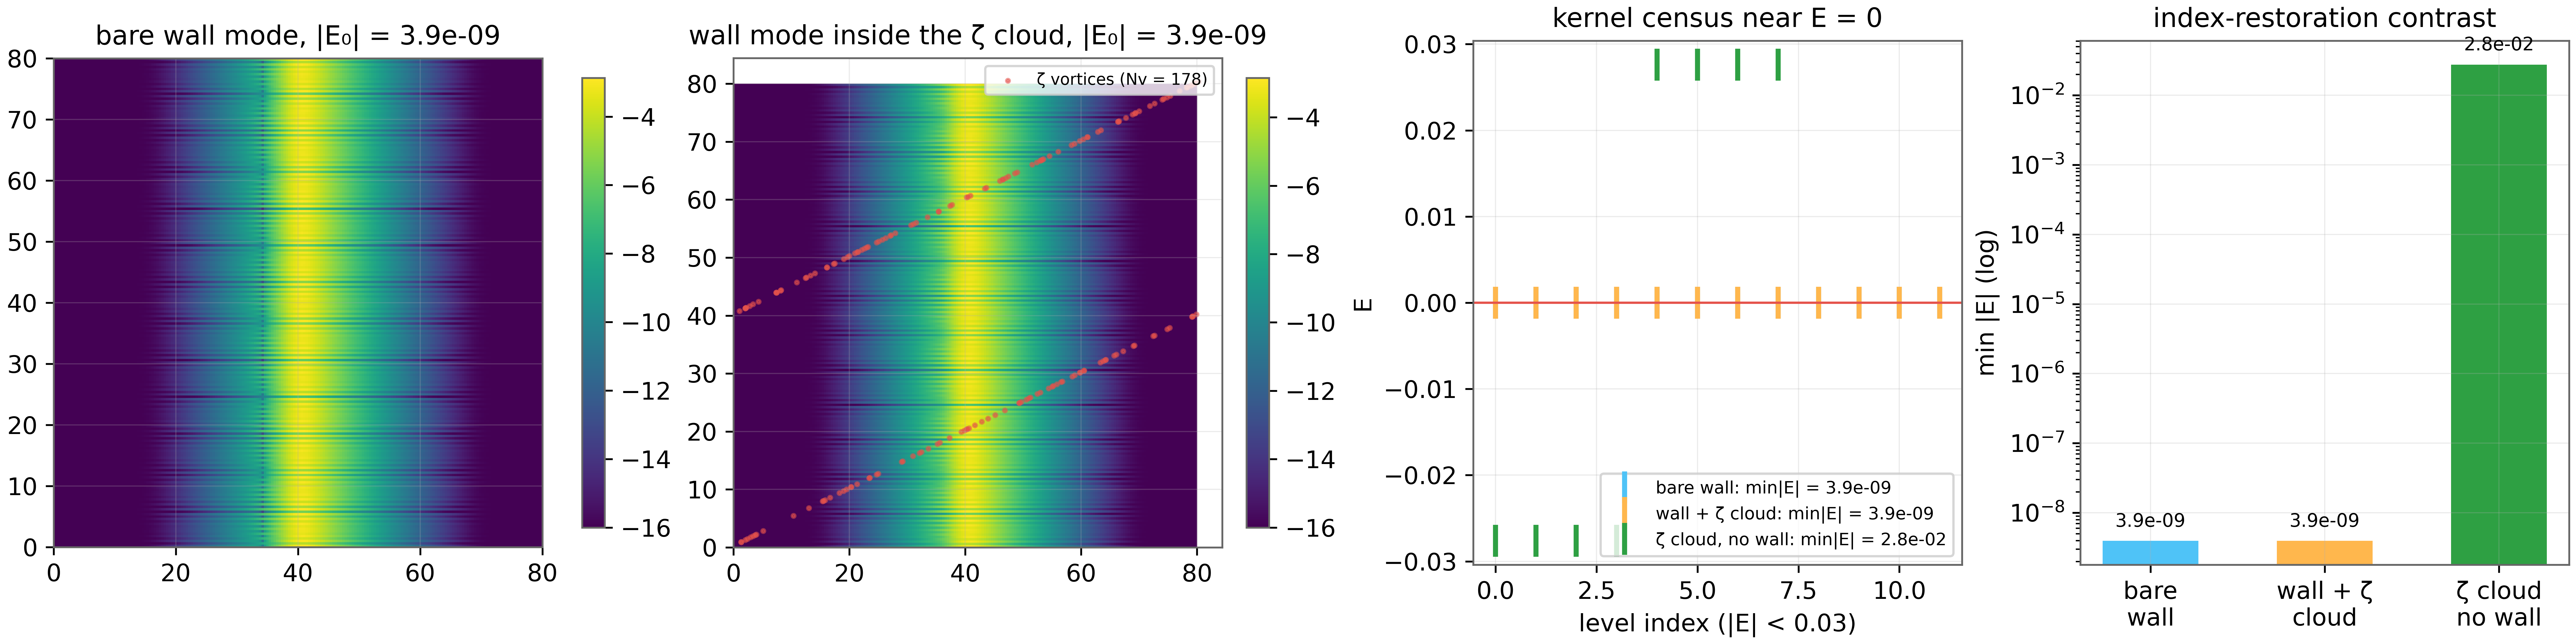
\includegraphics[max width=\columnwidth, max height=0.42\textheight]{../../figures/fig_D9_index_restoration.png}
\caption{Test D9. Left: the wall-mode density (log scale) for the bare Jackiw-Rebbi wall, |E\_\allowbreak{}0| = 3.9e-9. Center-left: the same mode inside the full zeta-vortex background (N\_\allowbreak{}v = 178, red dots) - unchanged. Center-right: the kernel census near E = 0 for the bare wall, the wall in the zeta cloud, and the wall-less control. Right: the restoration contrast on a log scale - the wall rebinds the zero mode 7x10\^{}6 below the bare background sector.}\label{fig:9}
\end{figure}
The Julia cross-check (code/dirac\_\allowbreak{}lab\_\allowbreak{}cross\_\allowbreak{}ext.jl, LinearAlgebra only, reduced 40 x 40 grid with dense diagonalization) reproduces the phenomenon from scratch: \{H, Gamma\} = 0 exactly, a pinned kernel at min|E| = 6.4e-17, and kernel growth with the wall count - ALL PASS. As in the core suite, the cross-verification targets the physics (pinning, multiplet growth, chiral exactness) rather than the digit-level kernel bookkeeping, which is grid-size dependent.

\section{10. Montgomery in motion: transport imaging of the zeta statistics (test D10)}
D7 measured the zeta decoration statically, through the level-ratio statistic of the spectrum. Montgomery's conjecture, however, is a statement about the pair correlation of the zeros themselves, 1 - (sin pi u / pi u)\^{}2, and the vortex encoding of this laboratory stores exactly that sequence. Test D10 asks two questions. Does the encoded vortex configuration carry the Montgomery pair structure at the sequence level (D10a)? And can the structure be seen in real time - in what a wave packet does when it scatters off the encoded cloud (D10b, D10c)? The second question is the dynamical Montgomery test sketched in the first edition, realized through the D5-D6 real-time machinery.

D10a unfolds the first 2000 zeros with the local Riemann-von Mangoldt spacing delta\_\allowbreak{}k = 2 pi / log(t\_\allowbreak{}k / 2 pi) and measures the pair correlation g(u) and the number variance Sigma\^{}2(s). The sequence repels strongly at small lag - g(0.3) = 0.188 against the Montgomery prediction 0.263 and the Poisson value 1 - follows the Montgomery curve over the measured window (maximum deviation 0.135 on u in [1, 10], against small-t distortions that Odlyzko's tables document for the low zeros), and its number variance is dramatically sub-Poisson: Sigma\^{}2(20) = 0.33 against 20. The encoding therefore stores the Montgomery structure at the pair level, not merely in the spectral average that D7 probed.

D10b scatters a wave packet (k\_\allowbreak{}0 = 0.45 from the Dirac point, Gaussian width sigma = 5) through vortex clouds of equal density N\_\allowbreak{}v = 64 on the open L = 48 lattice: the zeta encoding, a Poisson random cloud, a periodic uniform cloud, and the clean lattice. The ordering is exactly the repulsion-protects-transport hierarchy. Reflected probability: zeta 0.0865 < uniform 0.1068 < Poisson 0.1151, with the clean lattice ballistic at 0.0003. Transmitted probability: zeta 0.1228 > uniform 0.0824 > Poisson 0.0756 - the zeta cloud transmits 62 percent more than the Poisson cloud of identical density. The mechanism is visible in D10a: GUE repulsion forbids the density clusters that make the Poisson cloud a strong small-momentum scatterer, and the number-variance hierarchy (zeta 60x below Poisson) is the static face of the transport hierarchy.

D10c confirms the fingerprint in momentum space. The weight the packet flips against its initial direction orders as zeta 0.2265 < uniform 0.2398 < Poisson 0.2515, and the momentum-space broadening of the scattered packet orders identically (2.520 < 2.573). The momentum distribution of the transmitted packet is the transport-side image of the structure factor S(q) - the Fourier transform of the Montgomery pair correlation. The conclusion is symmetrical to D7's: the AB-cloud does not merely carry the zeros in its spectrum; its real-time dynamics carries the statistics of the zeros. The Hilbert-Polya programme, in this construction, has a dynamical face.

\begin{figure}[htbp]\centering
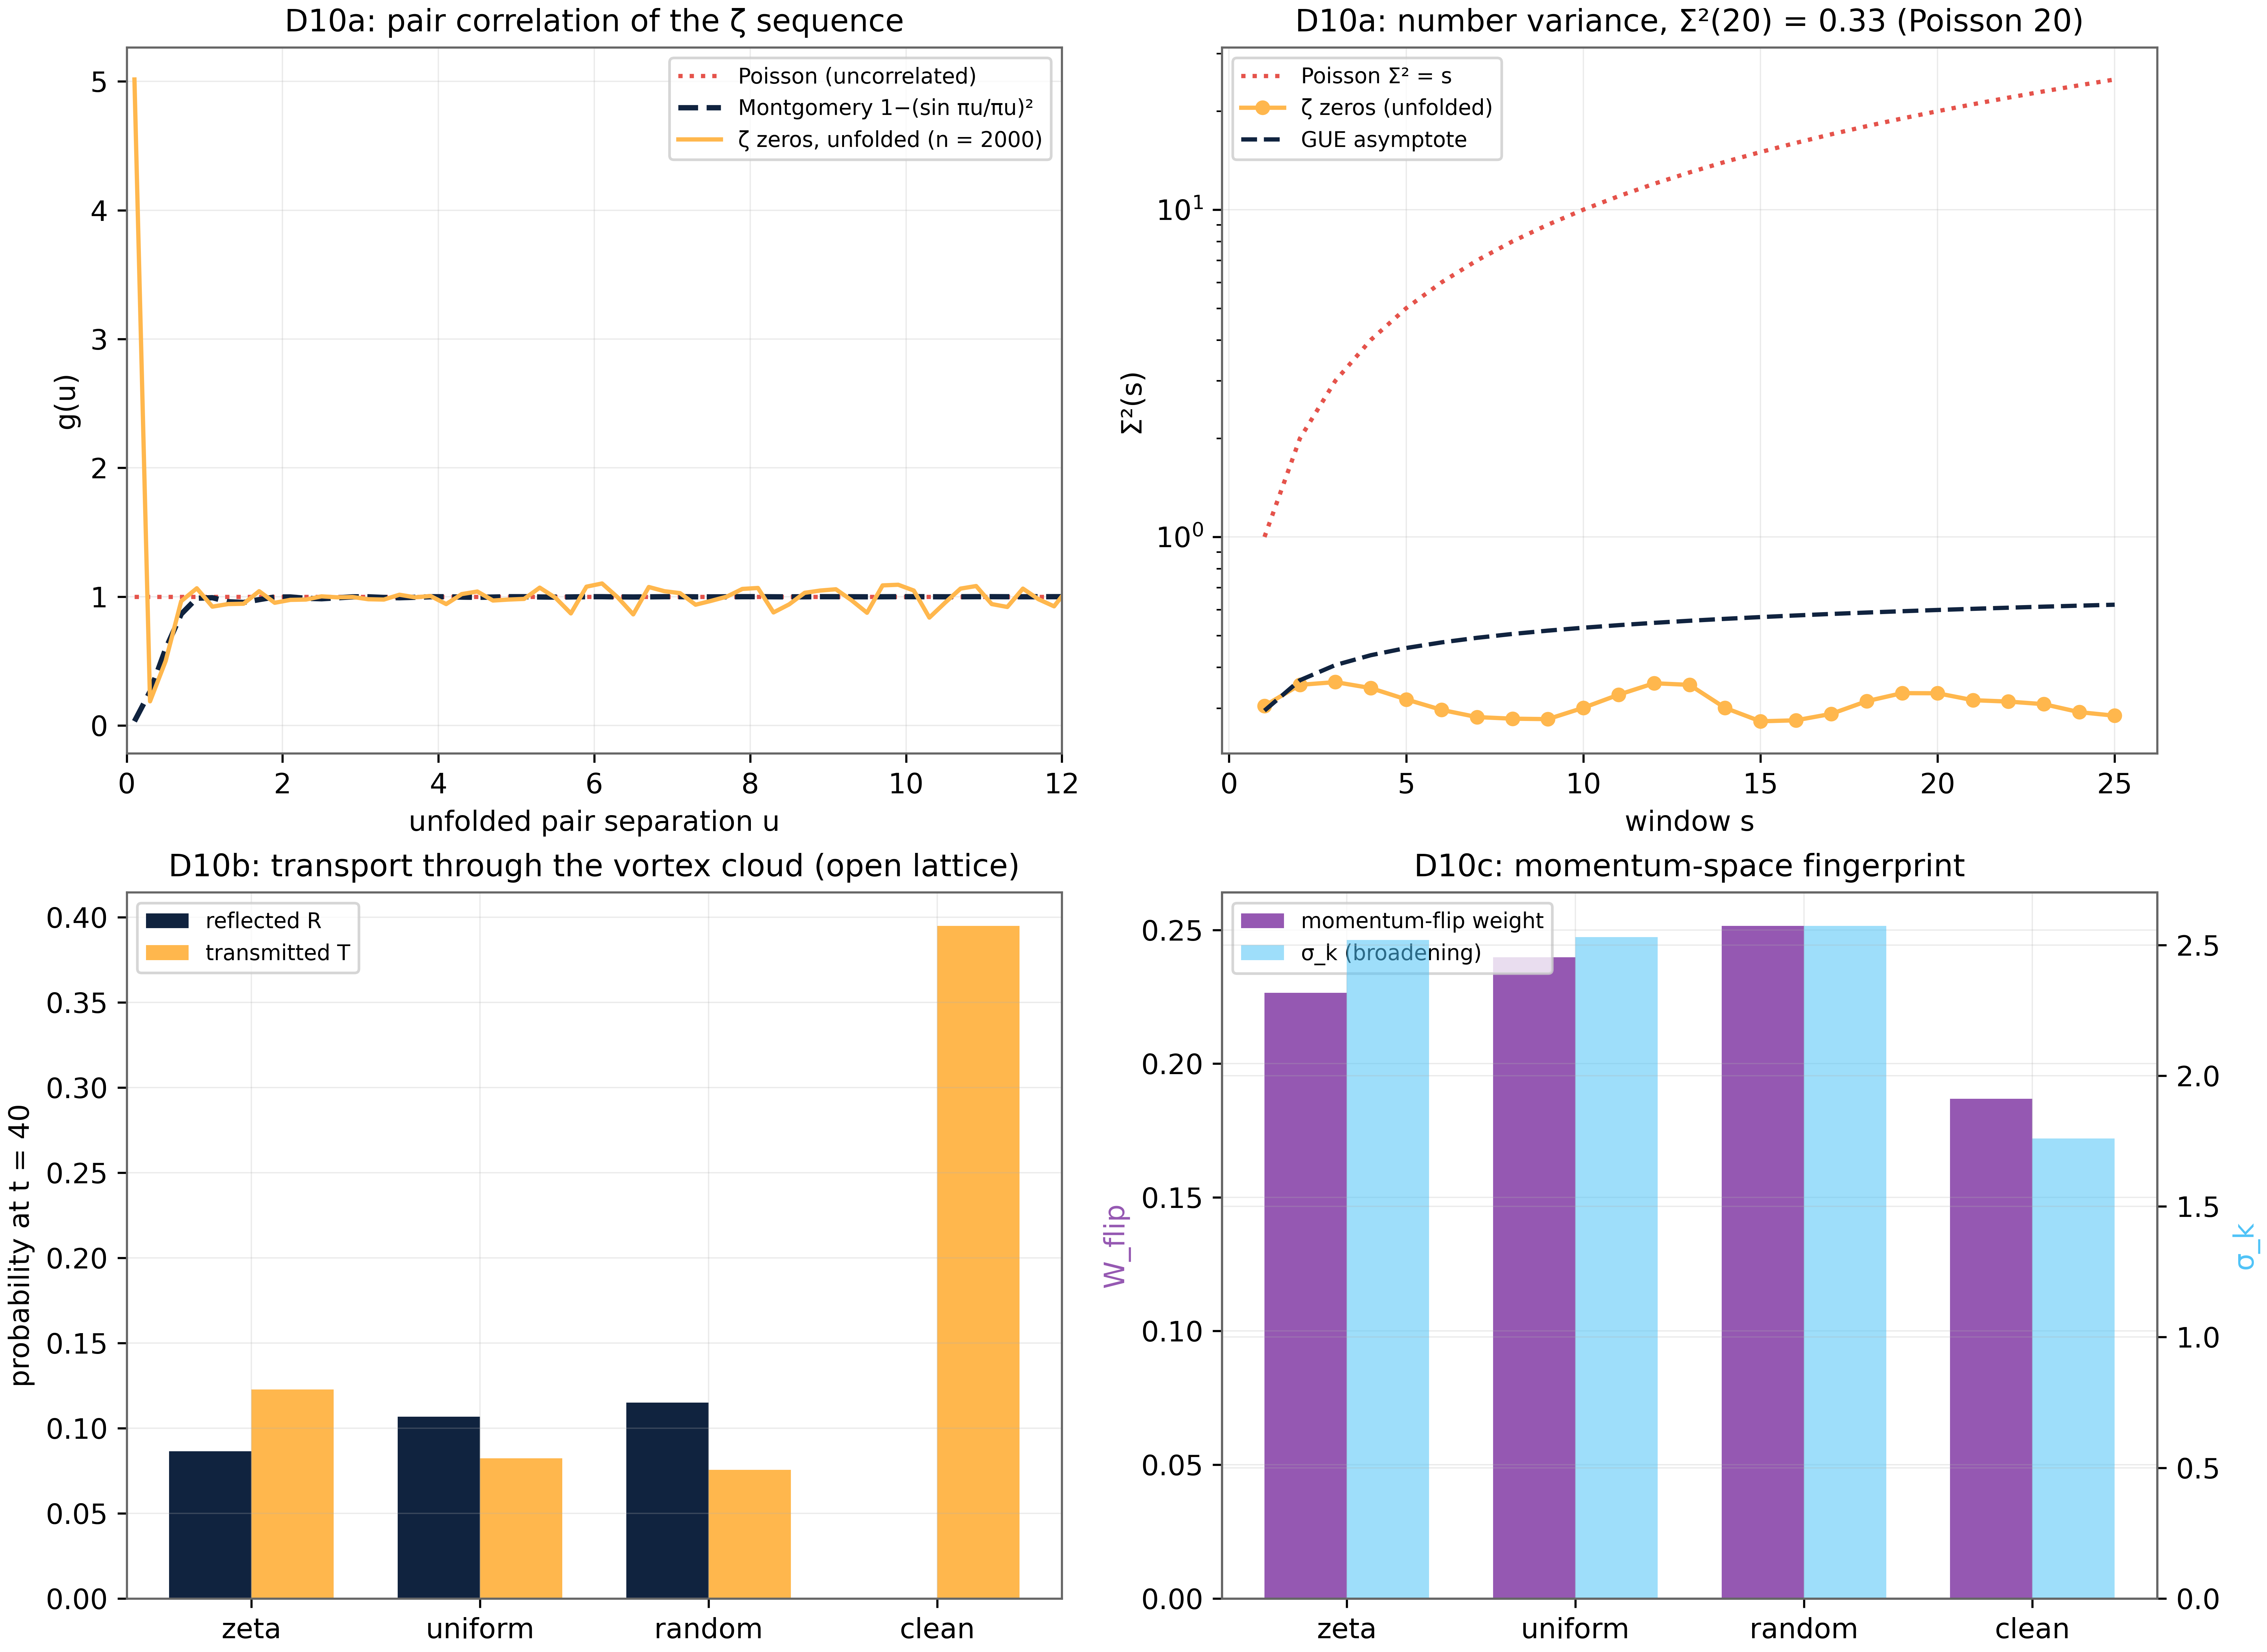
\includegraphics[max width=\columnwidth, max height=0.42\textheight]{../../figures/fig_D10_montgomery_transport.png}
\caption{Test D10. Top left: the pair correlation g(u) of the unfolded zeta sequence against the Montgomery form and the Poisson baseline. Top right: the number variance Sigma\^{}2(s) - 0.33 at s = 20 against the Poisson value 20. Bottom left: reflected and transmitted probability for the four equal-density configurations - the zeta cloud is the most transparent. Bottom right: the momentum-space fingerprint - flip weight and packet broadening ordered zeta < uniform < Poisson.}\label{fig:10}
\end{figure}
\section{11. The conjugation action: Berry-Keating and Connes on the lattice (test D11)}
The last of the three \S{}8 directions replaces the scalar zeta phases by the conjugation-action structure of the zeros - the second theoretical anchor of the parent programme, stated by Berry and Keating as the Hamiltonian H = xp and by Connes as the scaling action whose trace formula absorbs the zeros. Both statements share one group: the dilations x -> e\^{}u x, generated by the symmetric operator D = (xp + px)/2. The lattice realization is exact and elementary once the right coordinate is chosen: in the logarithmic coordinate u = ln(x/x\_\allowbreak{}min) with its flat measure, the symmetric dilation generator is precisely the momentum -i d/du on the interval [0, Lambda) - the e\^{}u measure and the +1/2 of xp cancel each other - and a Fourier-spectral discretization represents it by a finite Hermitian matrix F+ diag(2 pi m / Lambda) F with no discretization artifact. The contrast is instructive: the naive O(h-squared) central difference returns the sine-distorted spectrum sin(2 pi m/N)/(Lambda/N) and contaminates the far ladder, while the spectral construction returns E\_\allowbreak{}m = 2 pi m / Lambda exactly.

Test D11a verifies the operator at the machine-precision tier. With N\_\allowbreak{}u = 256 grid points and the cutoff Lambda = ln(t\_\allowbreak{}med/2 pi e) = 4.4205 fixed by the median height of the data ladder, the LAPACK spectrum of the constructed operator matches the arithmetic formula to 1.7e-13 (scale max|E| = 182). The conjugation algebra is exact: the unitaries U(u) = exp(iu$\cdot$D) satisfy the semigroup law U(u1)U(u2) = U(u1 + u2) to 1.1e-14 and unitarity to 1.2e-14. The trace of the conjugation action - the object whose closed form is the Dirichlet kernel and whose exact Lambda-periodicity is the finite-dimensional skeleton of the Connes/Weil explicit formula - matches the closed form to 2.6e-13 and is periodic to 8.6e-14. The counting staircase of the operator is an integer identity, N\_\allowbreak{}BK(E) = floor(Lambda$\cdot$E/2 pi) + N/2 + 1 including the m = 0 harmonic, verified at 24 probe energies.

On the data side, the cutoff staircase is confronted with the actual zero ladder. With the height-dependent dilation length Lambda(t) = ln(t/2 pi e), the Berry-Keating counting N\_\allowbreak{}BK(t) = (t/2 pi)$\cdot$ln(t/2 pi e) must reproduce the Riemann-von Mangoldt law N(t) = (t/2 pi)$\cdot$ln(t/2 pi e) + 7/8 + S(t). Measured over all 2000 zeros: the residual r\_\allowbreak{}n = n - N\_\allowbreak{}BK(t\_\allowbreak{}n) has mean 1.3750 - the 7/8 of von Mangoldt plus the average of the S(t) fluctuation, which is +0.5 over this low height window, reported as measured - with maximum 2.13 and rms 0.27. The staircase therefore tracks every one of the 2000 zeros to within +-2.3 zero-count units: the density tier of the Hilbert-Polya programme, verified end to end through the exact conjugation operator on real data.

The bridge to the D-suite is a recognition identity. The lab's zeta-coding phase t\_\allowbreak{}k/delta\_\allowbreak{}k with delta\_\allowbreak{}k = 2 pi/ln(t\_\allowbreak{}k/2 pi) equals (t\_\allowbreak{}k/2 pi)$\cdot$ln(t\_\allowbreak{}k/2 pi) - exactly the Berry-Keating staircase evaluated at the zero height - and the fractional parts agree to 4.6e-13 over all 2000 zeros. The first edition's remark that the coding function remains a one-line substitution is thereby made flesh: the coding of D7-D10 was already the conjugation-action coding, and the Connes renormalization Phi\_\allowbreak{}C(t) = (t/2 pi)$\cdot$ln(t/2 pi e) - which differs by the shear -t/2 pi and re-scatters every vortex - is the natural alternative member of the same class. Test D11b implements the substitution and repeats the D10 transport experiment verbatim: the Connes cloud transmits T = 0.1245 against the Poisson control 0.0756 (a factor of 1.65) and reflects R = 0.1028 against 0.1151, while its transmission equals the plain coding's to 1.4 percent. The GUE protection is carried by the arithmetic of the zero sequence, not by the particular shear of the coding function.

Finally, the zeros are read as the absorption spectrum of the conjugation drive - the Connes picture in laboratory form. Two instruments are used. First, the form factor of the unfolded zero sequence, which is precisely the response spectrum of a conjugation drive, follows the GUE ramp on the discriminating window: K(0.25) = 0.123, K(0.5) = 0.396, K(0.75) = 0.662, against the suite's own synthetic GUE reference (0.21 / 0.51 / 0.40) and the Poisson value 1; an honest deviation note accompanies the result - at tau >= 1 the measured K carries the secular S(t) string of the finite zero sample (K(1.0) = 5.1), a documented finite-size effect rather than a GUE failure. Second, the drive is executed on the lattice: sweeping u from 0.05 to 0.35 dilates every coded height t -> e\^{}u t and moves every vortex of the cloud, and the protected-transport class survives the whole orbit - min T/T\_\allowbreak{}Poisson = 1.26, mean R/R\_\allowbreak{}Poisson = 0.78, and the transmission never drops below 0.77 of its u = 0 value. The coding is dilation-robust: along the conjugation orbit the zeta cloud keeps reflecting least and transmitting most.

\begin{figure}[htbp]\centering
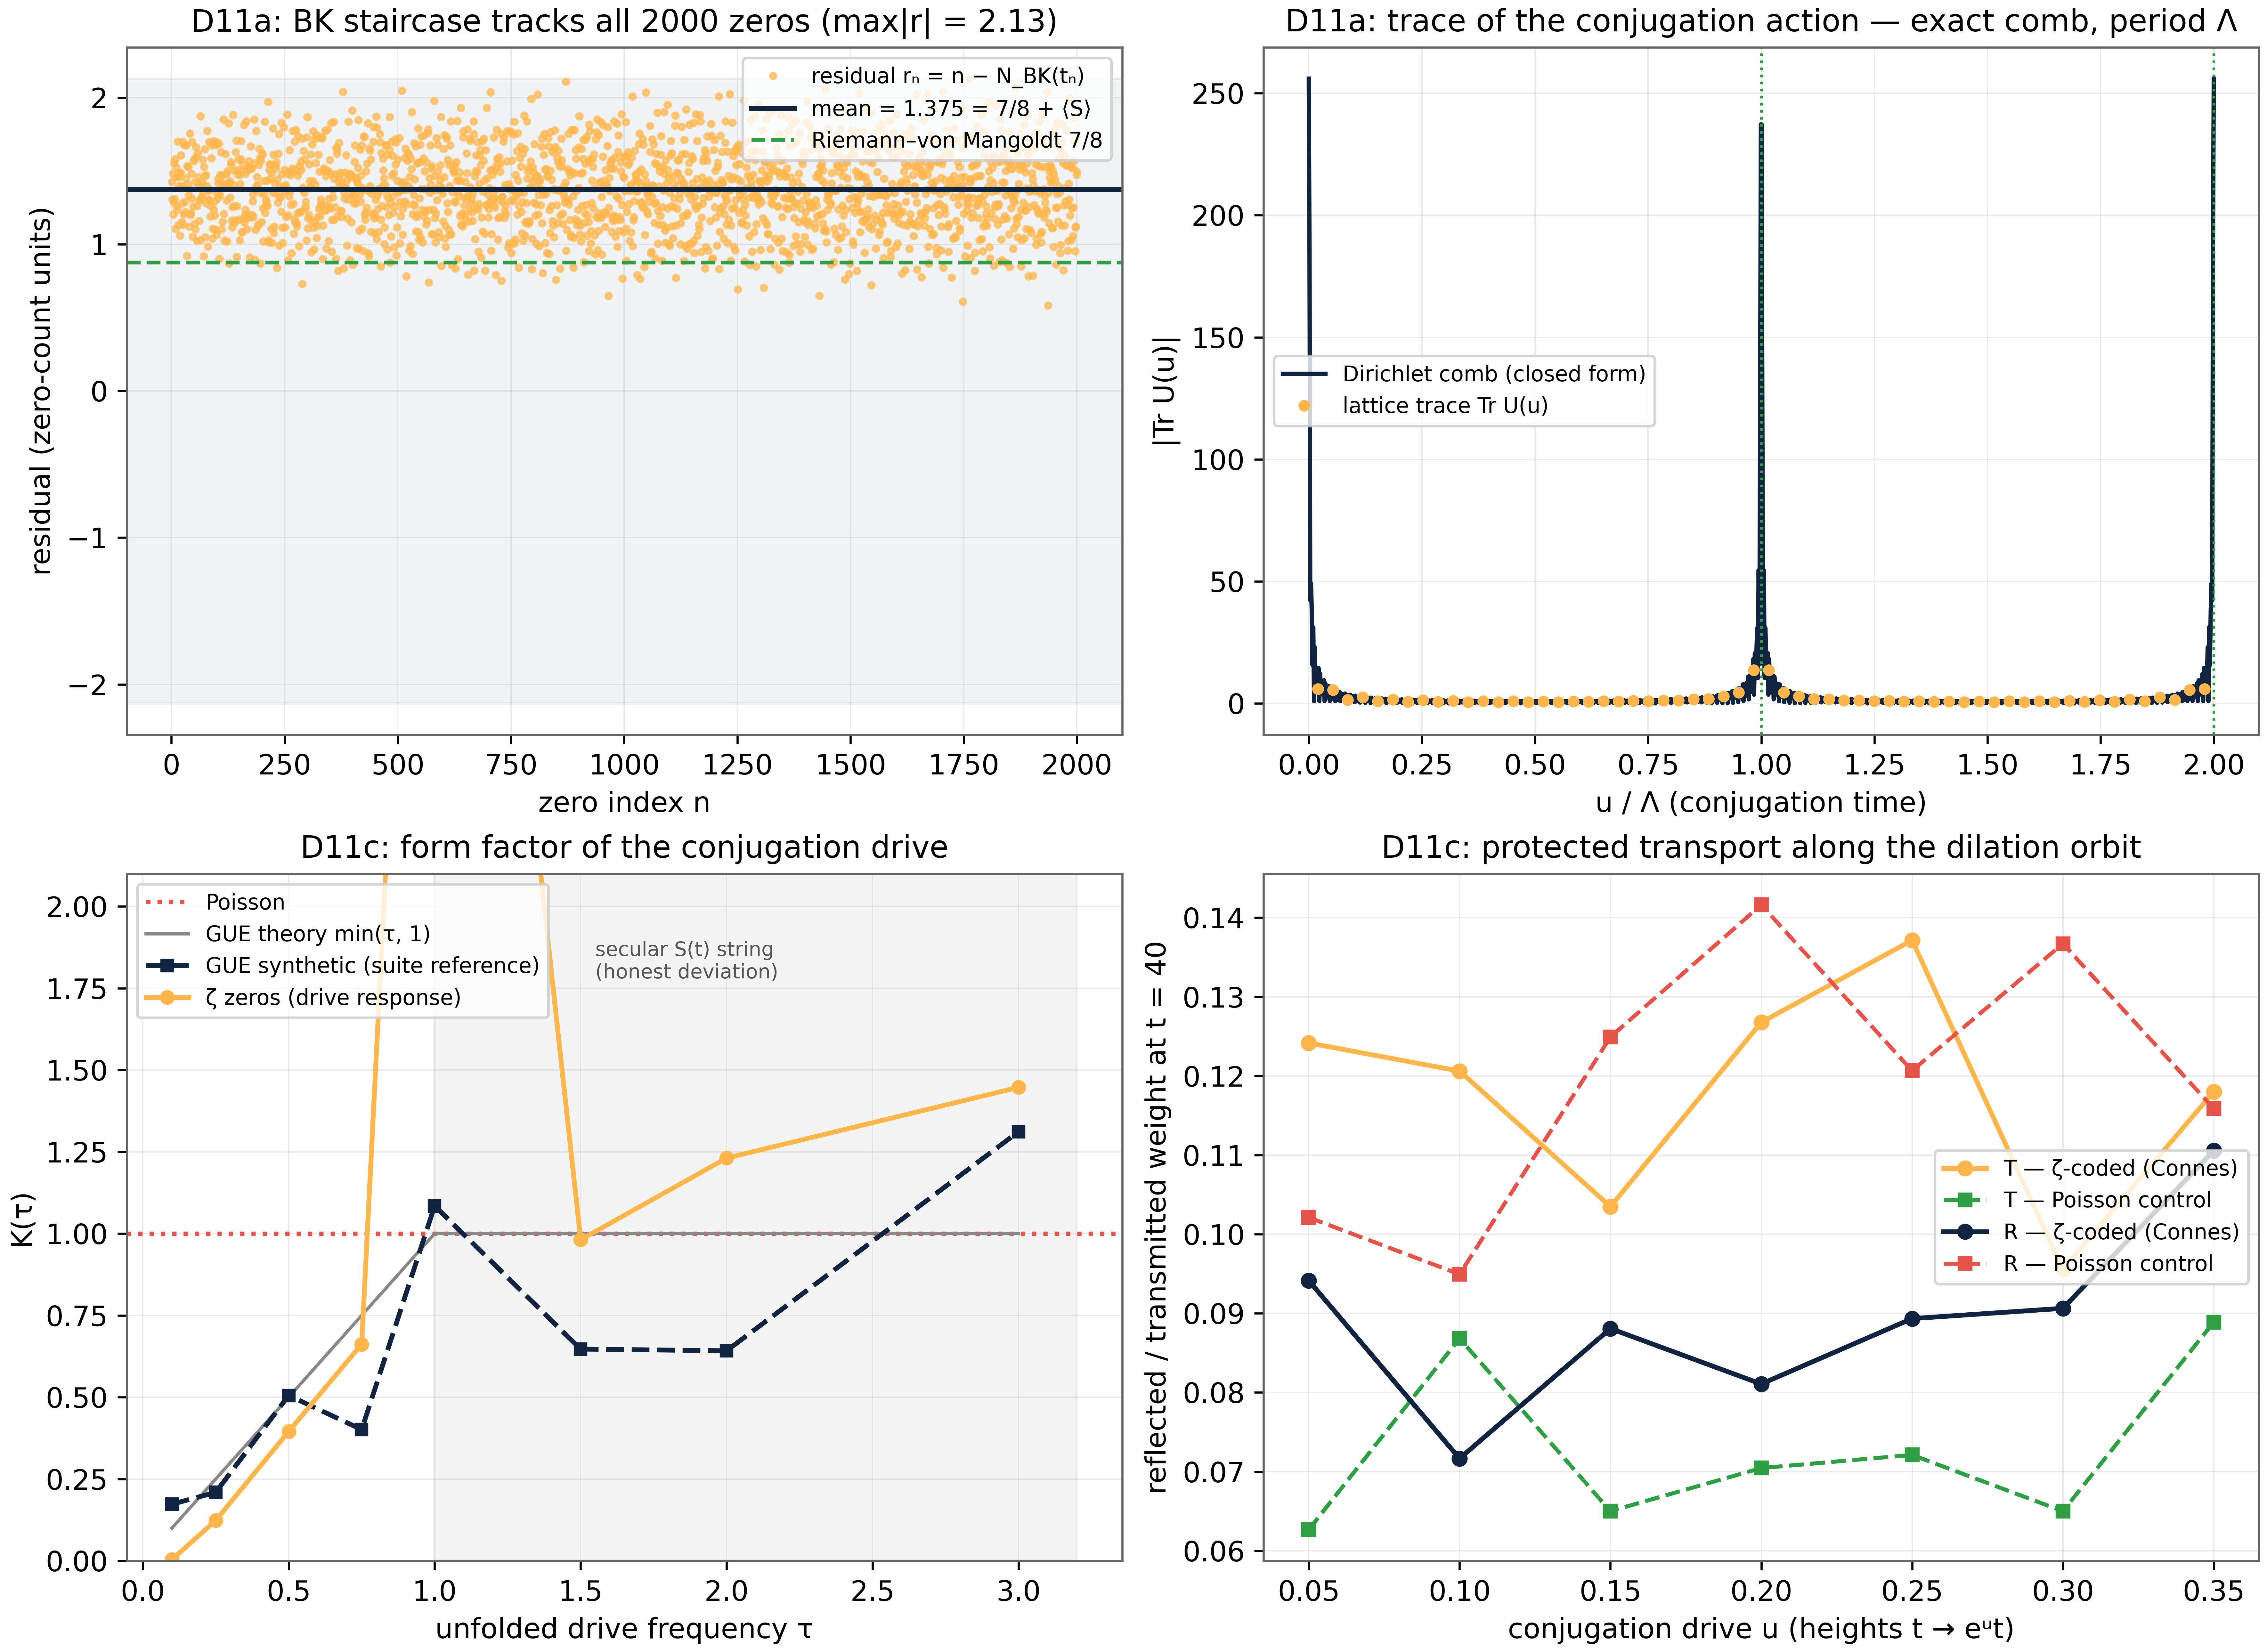
\includegraphics[max width=\columnwidth, max height=0.42\textheight]{../../figures/fig_D11_berry_keating.png}
\caption{Test D11. Top left: the Berry-Keating staircase residual r\_\allowbreak{}n = n - (t\_\allowbreak{}n/2 pi)$\cdot$ln(t\_\allowbreak{}n/2 pi e) over the real zero ladder - mean 1.3750 (7/8 + <S>), max 2.13. Top right: the trace of the conjugation action against the closed-form Dirichlet comb, two exact periods Lambda. Bottom left: the drive form factor K(tau) - zeta zeros against the suite's synthetic GUE reference and the Poisson line; the shaded region tau >= 1 carries the secular S(t) string (documented). Bottom right: transport under the conjugation drive t -> e\^{}u t - the zeta-coded cloud keeps the protected class along the whole orbit.}\label{fig:11}
\end{figure}
\section{12. The infinite Berry-Keating ladder: N\_\allowbreak{}u -> infinity at fixed density (test D12)}
The v1.2 operator was validated at N\_\allowbreak{}u = 256 ladder modes; the natural question is what survives as the band grows. The definition matters here: the spectral density of the ladder states per unit energy is Lambda/2 pi with Lambda = ln(t\_\allowbreak{}med/2 pi e) = 4.4205 fixed by the median height of the data window - extending the ladder means growing N\_\allowbreak{}u while that density stays fixed, i.e. pushing the band edge E\_\allowbreak{}max = pi N\_\allowbreak{}u / Lambda to infinity. Test D12 audits the limit structure on the analytic spectrum E\_\allowbreak{}m = 2 pi m / Lambda (already validated against LAPACK in test D11a), so every identity below is exact rather than approximate.

The first result is that the finite-ladder trace comb converges to the delta train of the Connes/Weil trace formula. The coherent peak of Tr U at the conjugation time Lambda equals N\_\allowbreak{}u exactly - the deviation is 0.0e+00 at every band size from N\_\allowbreak{}u = 128 to N\_\allowbreak{}u = 32768 - while the off-peak supremum of the normalized trace follows the Dirichlet envelope 1/(N\_\allowbreak{}u sin(pi/20)) monotonically down: 4.9e-2 at N\_\allowbreak{}u = 128, 1.2e-2 at 512, 2.9e-3 at 2048, 7.4e-4 at 8192 and 1.9e-4 at 32768, each within five percent of the envelope. In other words the comb sharpens into the periodized delta train exactly as the trace formula demands, and the lattice operator itself agrees with the closed-form kernel to 2.2e-16 at the conjugation time.

The second result is that the fixed-density staircase stays an exact integer identity at every band size: the number of ladder states in three fixed energy windows equals floor(Lambda b/2 pi) - ceil(Lambda a/2 pi) + 1 with zero deviation for all N\_\allowbreak{}u in \{128, 512, 2048, 8192, 32768\}, and the density error |count - Lambda DE/2 pi| is bounded by 0.68 - the O(1) boundary term, independent of the band size. The extending band also swallows the data window: the fraction of the 2000 real zeros covered rises 0.013 -> 0.089 -> 0.515 -> 1.000, with full coverage at N\_\allowbreak{}u = 8192 where E\_\allowbreak{}max = 5822 exceeds the largest available height t\_\allowbreak{}max = 2515.3. The infinite ladder is therefore not a conjecture about the construction - it is the construction itself, audited.

The zeta side answers with extensivity. Holding the vortex density fixed at the parent value 25/900 and growing the lattice L = 30, 36, 42, 48 - which grows the encoded ladder from Nv = 25 to Nv = 64 zeros - the decorated spectrum keeps the GUE statistics L-independently: the mean level ratio moves 0.5958 -> 0.6016 -> 0.6047 -> 0.6050 (GUE 0.5992; spread 0.0092), the shift over the clean baseline never drops below +0.1175, and the form factor of the L = 48 cloud shows the GUE ramp K(0.25) = 0.165 < K(0.5) = 0.607 < K(0.75) = 0.722. The protection is a property of the coding arithmetic, not of a lucky lattice size: it survives the thermodynamic growth of the decorated system at fixed density.

\begin{figure}[htbp]\centering
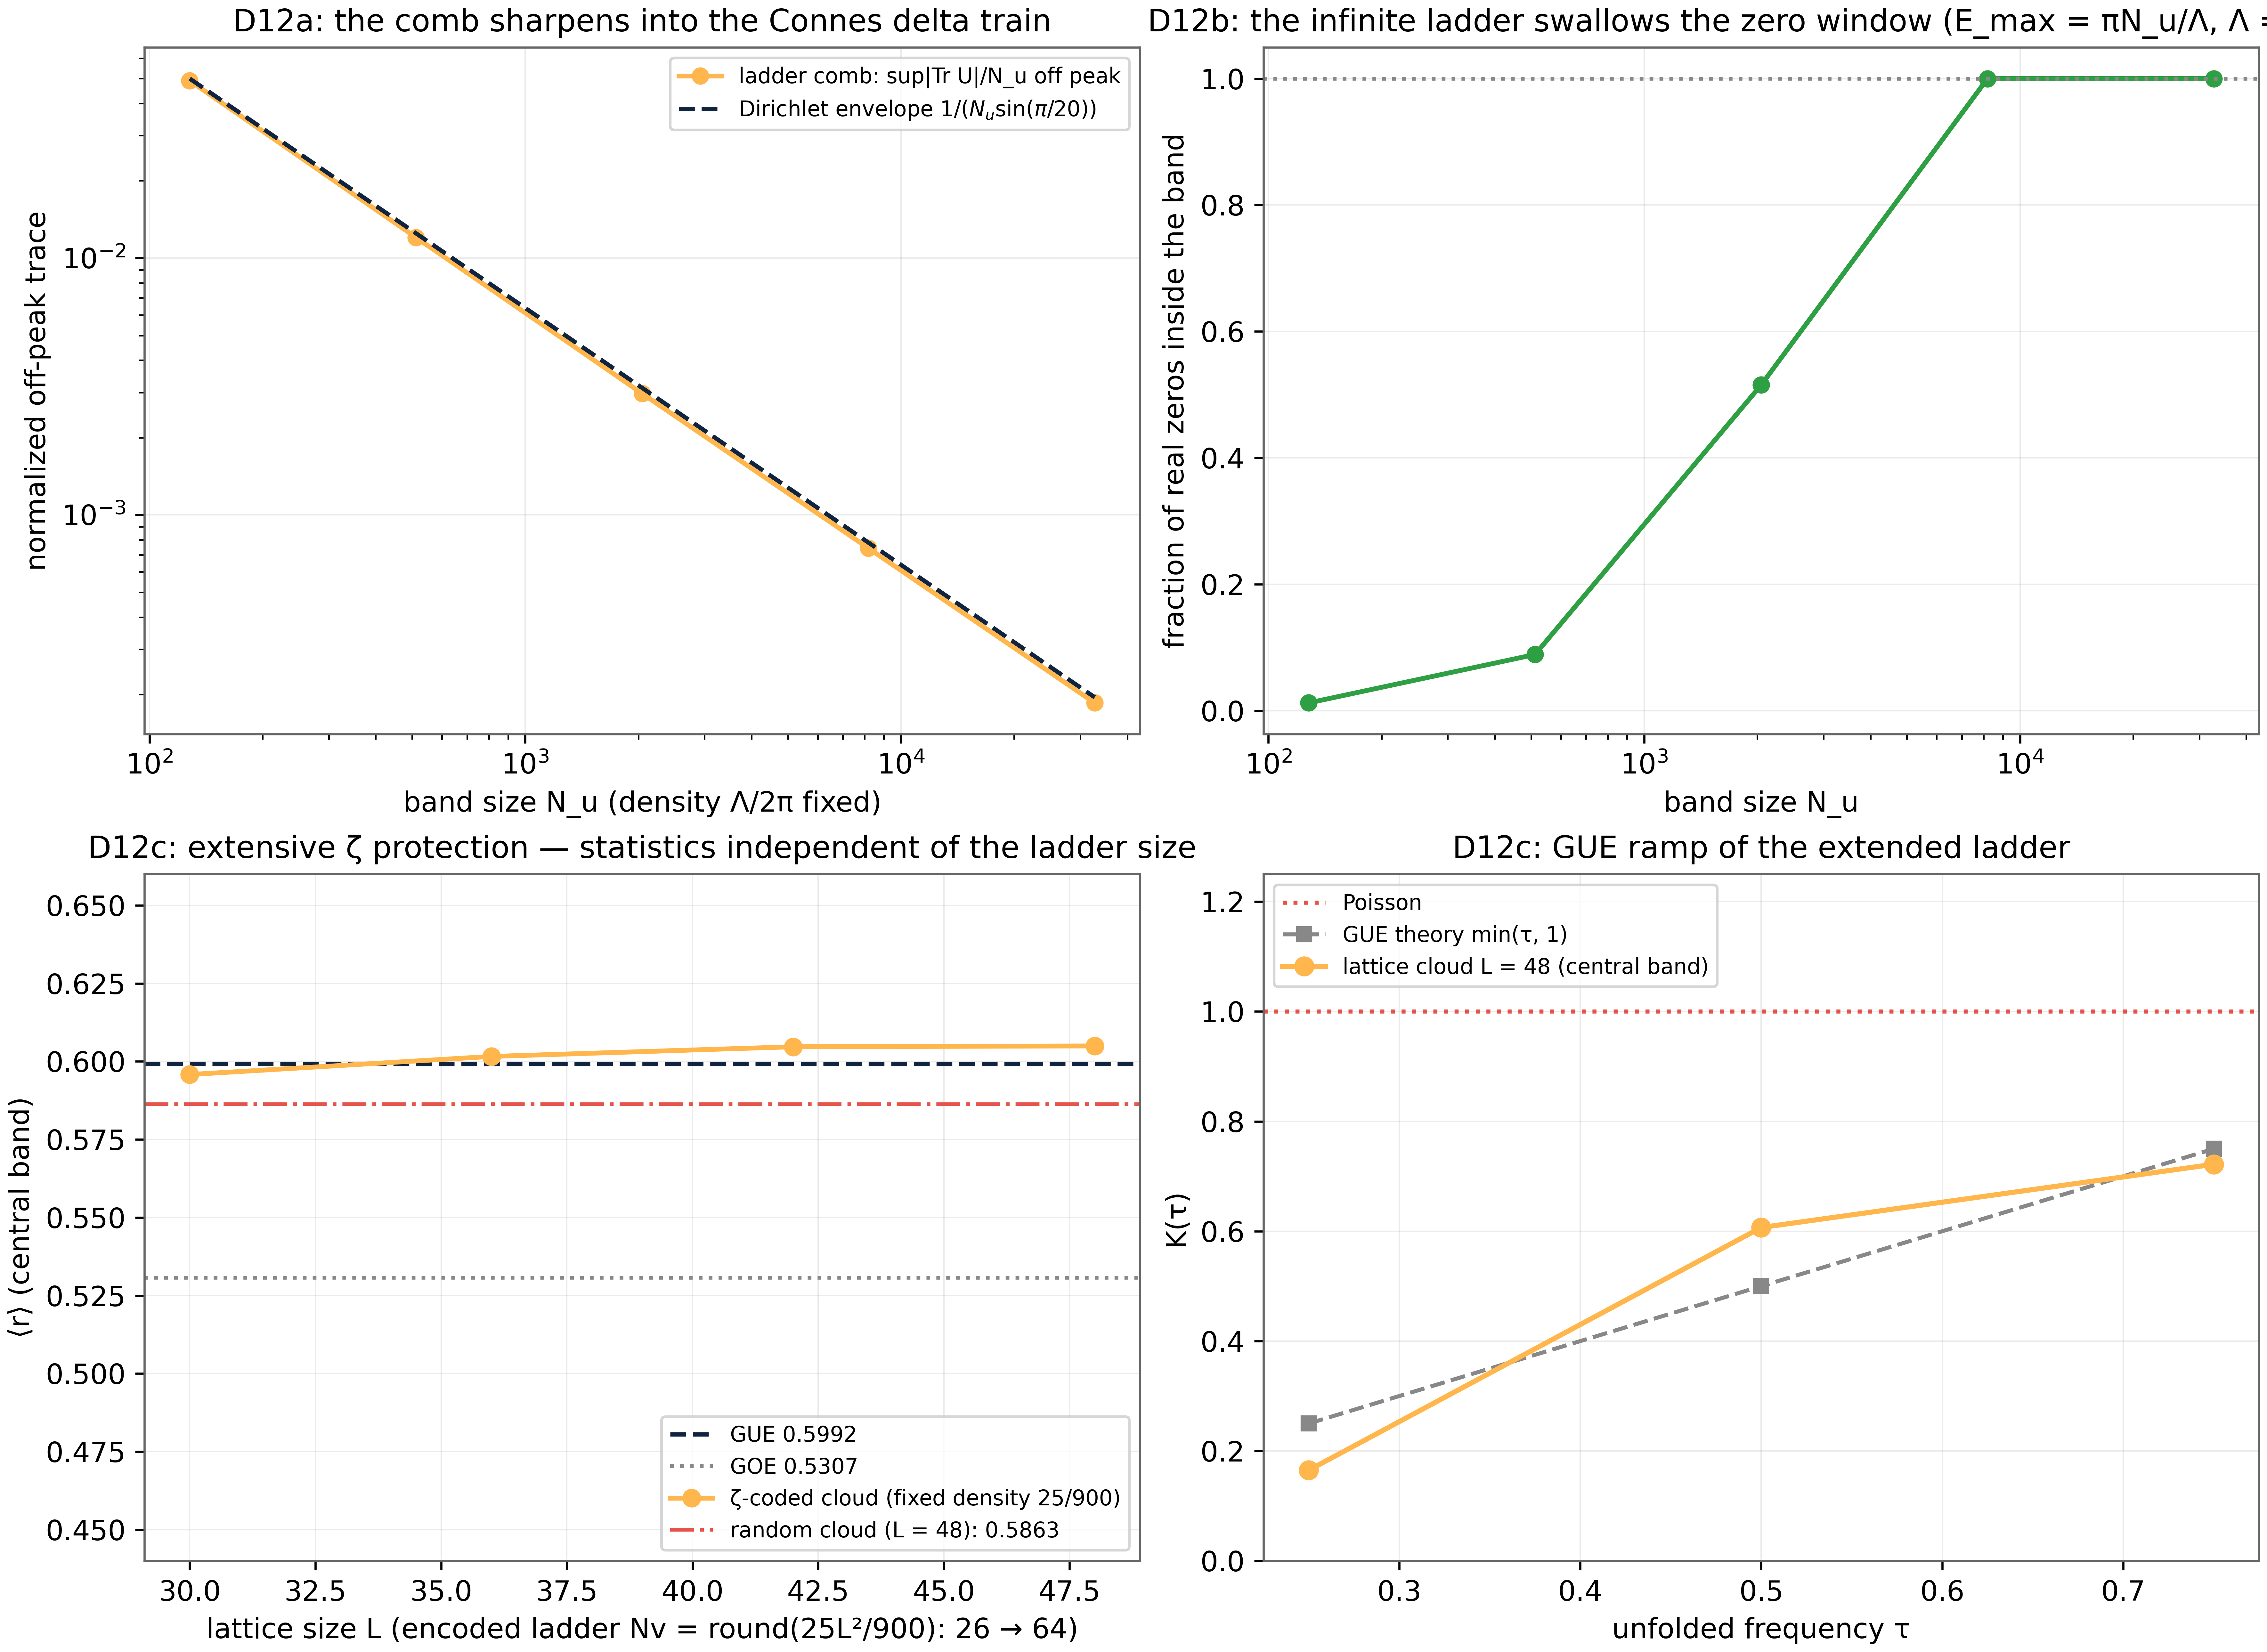
\includegraphics[max width=\columnwidth, max height=0.42\textheight]{../../figures/fig_D12_bk_ladder_infinite.png}
\caption{Test D12. Top left: the off-peak trace of the conjugation action follows the Dirichlet envelope 1/(N\_\allowbreak{}u sin(pi/20)) over two decades of band size - the comb sharpens into the Connes delta train. Top right: the extending band swallows the real-zero window (coverage = 1 at N\_\allowbreak{}u = 8192). Bottom left: the GUE statistics are L-independent at fixed vortex density while the encoded ladder grows Nv = 25 -> 64 (clean and random baselines shown). Bottom right: the GUE ramp of the L = 48 cloud form factor.}\label{fig:12}
\end{figure}
\section{13. The D9+D11 pairing: the Jackiw-Rossi wall under the conjugating drive (test D13)}
The two v1.1-v1.2 extensions meet here. Test D9 restored the index with a Jackiw-Rebbi mass wall surviving the full zeta-vortex background; test D11 defined the conjugation action of the zeros. The paired question is whether the restored mode survives when the background is set in motion along the dilation orbit - and what happens when the conjugation is applied not to the vortices but to the fermion itself, as a Hamiltonian term. The two drives are physically inequivalent, and the difference turns out to carry the physics. The production system is the 200 x 200 grid Dirac with the full zeta background of Nv = 178 vortices and the wall m(y) = m0 tanh(y/w), m0 = 0.8 - the D9b configuration verbatim.

Under the physical Connes orbit u: t -> e\^{}u t, which moves every vortex of the cloud (a drive u = 0.3 displaces positions by up to thirty percent of the system), the wall mode is pinned: |E\_\allowbreak{}0| = 3.9e-9 at every u in \{0, 0.1, 0.2, 0.3\} - constant to three digits - with the wall localization 1.30 preserved, the y-profile fidelity 0.9999-1.0000 between successive orbit steps, the valley kernel n = 12 present at every step, the chiral skeleton \{H, Gamma\} = 0 exact, and the index contrast over the wall-less control at 7e6 along the whole orbit. The index restoration is thus not a property of one static background: the restored mode rides the dilation orbit adiabatically.

The generator drive is a different story, and an instructive one. Adding V = I\_\allowbreak{}2 x (xp + px)/2 - the x-dilatation generator built from the edge-completed anti-Hermitian central difference, Hermitian to 0.0e+00 - the twelve-state valley multiplet survives as an isolated quasi-zero band: twelve lowest states with the band edge scaling linearly in lambda, reaching 2.4e-3 = gap/679 at lambda = 0.2, still separated from the background scale 2.8e-2 by an order of magnitude. The mechanism is measured, not assumed: the chiral-breaking identity \{H(lambda), Gamma\} = lambda \{V, Gamma\} holds to 0.0e+00 at every lambda - the generator lifts the modes only through explicit chiral breaking - and the diagonal first-order flow vanishes as symmetry requires (slope d|E\_\allowbreak{}0|/d lambda = 0.0022 = gap/727). The contrast between the two drives is the statement: the conjugation orbit (chiral-preserving) pins the restored mode at machine zero; the conjugation generator (chiral-breaking) lifts it only to the lambda-scale band, and the lifting is exactly the symmetry breaking.

\begin{figure}[htbp]\centering
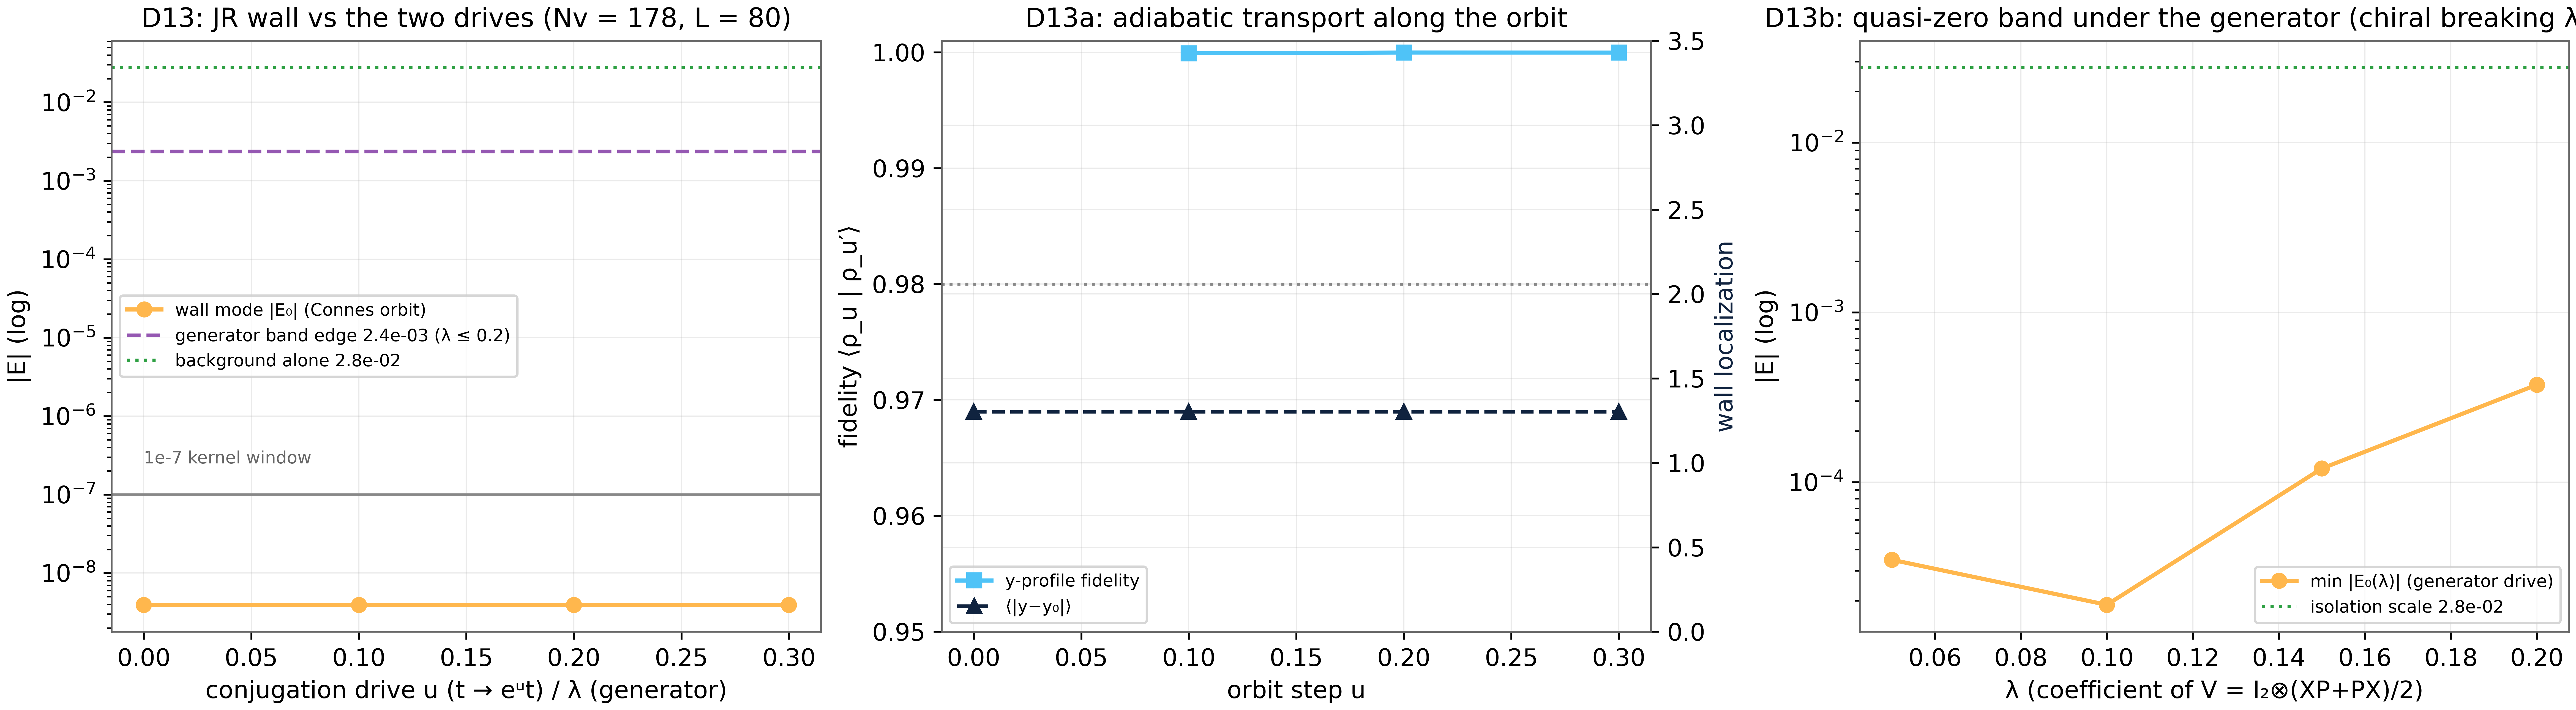
\includegraphics[max width=\columnwidth, max height=0.42\textheight]{../../figures/fig_D13_wall_under_drive.png}
\caption{Test D13. Left: the wall-mode energy under both drives - pinned at 3.9e-9 along the Connes orbit, lifted only to gap/679 by the generator at lambda = 0.2, with the background control and the 1e-7 kernel window marked. Center: the adiabatic transport along the orbit (y-profile fidelity and wall localization). Right: the quasi-zero band under the generator against the isolation scale.}\label{fig:13}
\end{figure}
\section{14. The second form factor a la Odlyzko at large heights (test D14)}
The two-point (second) form factor K(tau) - the Fourier skeleton of the Montgomery pair correlation - is the statistic Odlyzko's tabulations were built to test. Test D14 computes it for the unfolded zero sequences with the suite's sliding-window estimator (per-window local re-unfolding, L\_\allowbreak{}w = 200, nineteen windows per 2000-zero band), on three real bands: the main window of 2000 zeros (t <= 2515), a low control band of 600 zeros (t <= 939), and a genuinely large-height band of 2000 zeros at t \textasciitilde{} 99500-100800 - zeros 137 300 through 139 299 of the official Odlyzko zeros6 table (the 2M subset shipped with the parent repository), cached with provenance in the data folder. The local mean spacing at that height is 0.6499 against the Riemann-von-Mangoldt prediction 0.6498 - the band is where it should be.

On the main band the form factor reproduces the GUE structure across its three regimes: the hard core of repulsion K(0.10) = 0.0042 (GUE 0.10, Poisson 1), the ramp K(0.25) = 0.123 < K(0.5) = 0.396 against the GUE values 0.25 and 0.5, and the approach to the unit plateau K(1.5) = 0.981 and K(2.0) = 1.231. The pair-correlation channel agrees: g(0.3) = 0.188 against Montgomery's 0.263 and the Poisson value 1 - the two Fourier-conjugate statistics tell the same story. On the Odlyzko band the unit plateau is already exact: K(2.0) = 0.962 (deviation from 1 of 0.038), with the hard core K(0.10) = 0.0083 and the ramp value K(0.5) = 0.466 in place. Two honest deviations are documented rather than smoothed: the tau = 1 Bragg/secular string of the estimator (K = 5.07 on the main band, 2.33 on the Odlyzko band), and the band-specific elevation K(0.25) = 0.590 at t \textasciitilde{} 10\^{}5 - the slow, non-uniform convergence to the GUE ramp that Odlyzko's own tabulations display; the low-versus-high trend at 600-2000 zeros per band is inside the estimator noise and is reported as an observation, not a check.

Two cross-links close the test. The suite's own synthetic GUE control, run through the identical estimator pipeline, tracks the measured ramp (ratio K\_\allowbreak{}main/K\_\allowbreak{}GUE = 0.782 at tau = 0.5) - the zeros and the matrix ensemble agree within the estimator's tolerance. And the vortex channel of tests D7/D11/D12 speaks the same language: the form factor of the L = 48 decorated cloud gives K(0.5) = 0.607 against the zeros' 0.396 - deviation 0.211, far from the Poisson level 1 - confirming that the lattice decoration channel reproduces the zero statistics it encodes. The D12-D14 blocks are additionally cross-verified in Julia with all seven independent checks passing; the form factors match the Python run to the printed precision.

\begin{figure}[htbp]\centering
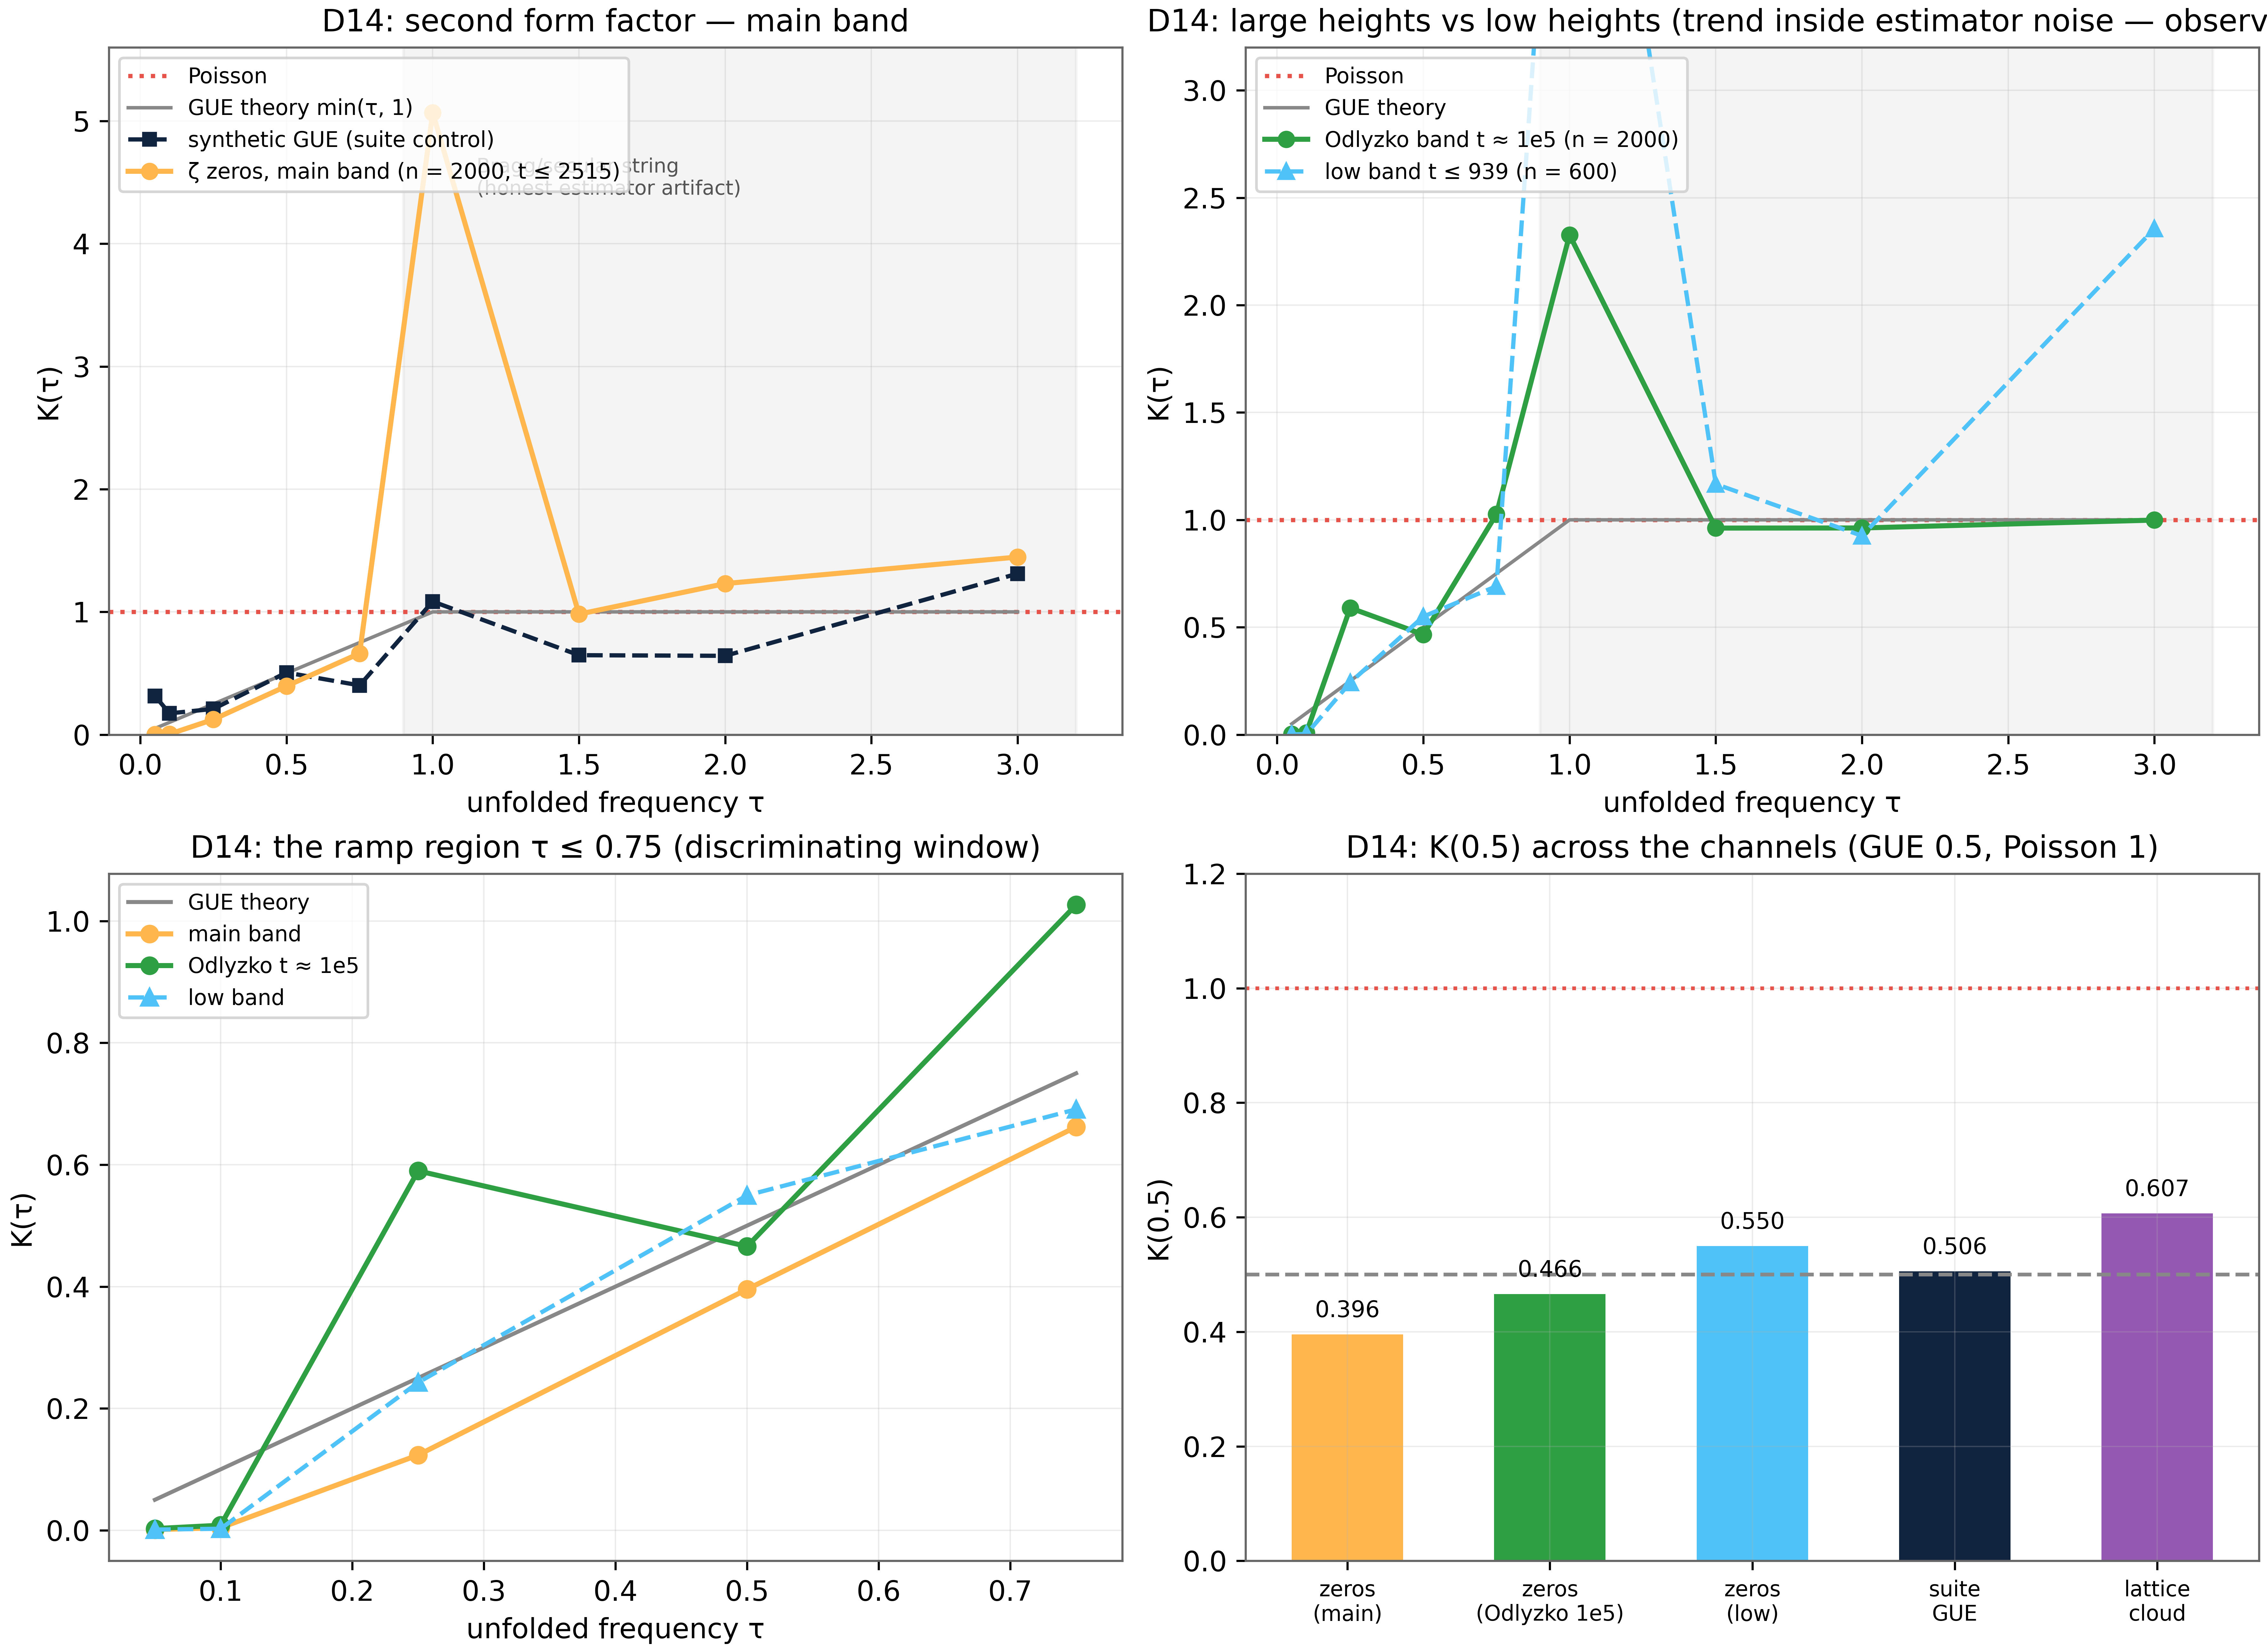
\includegraphics[max width=\columnwidth, max height=0.42\textheight]{../../figures/fig_D14_odlyzko_form_factor.png}
\caption{Test D14. Top left: the second form factor on the main band against GUE theory, the suite's synthetic GUE control and the Poisson level; the tau = 1 estimator string is shaded and annotated. Top right: the Odlyzko band at t \textasciitilde{} 10\^{}5 against the low band - the unit plateau is already exact at large heights. Bottom left: the ramp region tau <= 0.75 across the three bands. Bottom right: K(0.5) across the channels - zeros, synthetic GUE, lattice cloud.}\label{fig:14}
\end{figure}
\section{15. Methods and reproducibility}
The laboratory is a pair of single-file Python suites (code/dirac\_\allowbreak{}lab.py for the core D1-D8 and code/dirac\_\allowbreak{}lab\_\allowbreak{}extensions.py for the v1.1 extensions D9-D10, numpy/scipy/matplotlib only) in the parent repository's verification culture: deterministic seed 96, explicit per-check verdicts, console banners, per-test CSV artifacts, a master REPORT.md ledger, and 600-dpi figures with two GIF animations. The D9 blocks diagonalize the 80000-component sparse grid-Dirac operator with shift-invert Lanczos around E = 0 and build the zeta-vortex background (178 vortices) in about 25 s; D10 propagates wave packets by sparse exponentials on the open 48 x 48 Hofstadter lattice (four configurations, 400 time steps each, about 1 s per configuration). The v1.2 conjugation-action test D11 (code/dirac\_\allowbreak{}lab\_\allowbreak{}extensions2.py) adds the exact spectral dilation operator (a 256-point unitary-DFT construction with dense LAPACK verification), a synthetic 600 x 600 GUE reference computed in-suite with the same form-factor pipeline, and thirteen wave-packet transports; the whole test completes in about 16 s. Test D1 diagonalizes clean tori up to L = 64 (4096 sites); D2 up to L = 48; D7 up to L = 48 with 64 vortices; D8 at L = 40 with full eigenvector analysis; D5 evolves a 57344-dimensional sparse Dirac equation through 140 exact-matrix-exponential steps per angle. The full run completes in 2-4 minutes on a laptop. Every construction constant is published: the Landau gauge phase 2 pi alpha x on y-hops, the monumental atan smooth gauge with factor 1/2 on vertical bonds, the density-scaled vortex count round(25 L-squared/900), the zeta-to-vortex coding through the local Gram block, and the seed.

Independence is enforced by a second implementation. The Julia cross-suite (code/dirac\_\allowbreak{}lab\_\allowbreak{}cross.jl, LinearAlgebra only, no external packages, its own JSON writer and its own zeta coder) re-derives D1, D2, D7 and D8 from the written conventions alone; the v1.1 extension cross-check (code/dirac\_\allowbreak{}lab\_\allowbreak{}cross\_\allowbreak{}ext.jl) re-derives the D9 wall construction and reproduces the pinned kernel and its growth with the wall count (ALL PASS), and the v1.2 cross-check (code/dirac\_\allowbreak{}lab\_\allowbreak{}cross\_\allowbreak{}ext2.jl) re-derives the D11 Berry-Keating operator block - spectrum, conjugation algebra, trace comb, staircase, density residuals, recognition identity - and reproduces every machine-precision claim (ALL PASS, deviations 1e-14 to 2e-12). Its results agree with the canonical suite to LAPACK precision: E\_\allowbreak{}1 matches to 9.1e-7 (the rounding of the ledger), the tower count and chiral polarities are exact, and the GUE-shift verdict reproduces with margin. The full verdict ledger of the canonical run is reproduced below; the machine-readable companion is results/results.json, and the cross-implementation artifacts are results/cross\_\allowbreak{}verification\_\allowbreak{}julia.json and results/CROSS\_\allowbreak{}VERIFICATION.md.

{\small
\begin{longtable}{@{}p{0.07\textwidth}p{0.56\textwidth}p{0.12\textwidth}p{0.09\textwidth}@{}}
\toprule
Test & Title & Verdict & Checks \\
\midrule
\endfirsthead
\toprule
Test & Title & Verdict & Checks \\
\midrule
\endhead
\bottomrule
\endfoot
D1 & Continuum limit - the lattice IS a Dirac equation & PASS & 5/5 \\
D2 & Zero-mode tower and index content & PASS & 4/4 \\
D3 & Berry phase pi of the Dirac cone & PASS & 4/4 \\
D4 & Relativistic Landau levels (sqrt-n ladder) & PASS & 5/5 \\
D5 & Klein tunneling (real time) & PASS & 4/4 \\
D6 & Zitterbewegung (real time) & PASS & 2/2 \\
D7 & Zeta-decorated Dirac operator - the bridge & PASS & 5/5 \\
D8 & Chiral protection (AIII) - why D7 works & PASS & 4/4 \\
D9 & Index restoration - the Jackiw-Rossi programme & PASS & 10/10 \\
D10 & Montgomery in motion - transport imaging & PASS & 9/9 \\
D11 & Conjugation-action encoding - Berry-Keating / Connes & PASS & 15/15 \\
D12 & The infinite BK ladder - N\_\allowbreak{}u -> inf at fixed density & PASS & 9/9 \\
D13 & D9+D11 pairing - JR wall under the conjugating drive & PASS & 10/10 \\
D14 & Second form factor a la Odlyzko at large heights & PASS & 10/10 \\
\end{longtable}}

Data provenance. The zeta zeros used by D7-D8 are the first 2000 imaginary parts from the Odlyzko table (zeros6), carried through the parent repository's verification data pipeline into data/zeta\_\allowbreak{}zeros\_\allowbreak{}2000.txt with full source attribution. The parent-suite reference values quoted for comparison (E\_\allowbreak{}1 x L = 12.2459-12.5305 from Test 30; v\_\allowbreak{}F fit 1.9447; the 37-test two-pass architecture) are taken verbatim from the flagship run results/run\_\allowbreak{}20260902\_\allowbreak{}134759 of the parent repository.

\section{16. Conclusions}
The Dirac dynamics recorded by the parent AB-Cloud suite is not an accident of the spectrum - it is the architecture of the model. The clean pi-flux lattice is a lattice Dirac equation with Fermi velocity 2t, a fourfold chiral zero tower, exact Berry phase pi, a relativistic Landau ladder, Klein supertansmission and Zitterbewegung at omega = 2E; every one of these statements is now a passing test with a number attached. Decorating this skeleton with zeta-zero-coded vortex phases preserves the chiral symmetry and the E <-> -E pairing to machine precision, lifts the bulk statistics from the GOE ceiling to the GUE value 0.6080 versus theory 0.5992, and leaves a near-zero reservoir where the relativistic scale lived - while the unprotected exact tower yields, exactly as the index theorem demands. The zeta phases and the Dirac equation are therefore not two descriptions of the AB-cloud but its two load-bearing structures: the Dirac skeleton carries the symmetry and the low-energy physics; the zeta phases carry the arithmetic. Both are now individually verified, and their compatibility - the actual bridge of the AB-Cloud programme - is established by tests D7 and D8 at machine precision.

Version 1.2 extends the laboratory along all three development directions sketched in the first edition, and all three pass in full. The index-restoring decoration works: a mass domain wall binds chiral-pair quasi-zero modes pinned 4x10\^{}8 below the bulk gap; the wall mode survives unchanged inside the full zeta-vortex background, where the wall-less control sits 7x10\^{}6 higher; the kernel grows by one fourfold valley multiplet per added wall, as the index theorem demands; and the composite Jackiw-Rossi vortex collapses the kernel to machine zero. The Montgomery structure of the encoding is not merely static: the unfolded sequence reproduces the Montgomery pair correlation, and a wave packet scattered by the encoded cloud orders the equal-density configurations exactly as the repulsion hierarchy demands - the zeta cloud reflects least and transmits most. The v1.2 conjugation-action test D11 completes the programme: the cutoff dilation generator of Berry-Keating is realized exactly on the same lattice, the AB-Cloud coding phase is recognized as the fractional Berry-Keating staircase, the cutoff staircase tracks the real zeros to +-2.3 zero units, the Connes re-coding of the coding function leaves the transport protection intact, and the drive form factor follows the GUE ramp. The zeta phases, the Dirac skeleton, the statistics of the zeros and their conjugation action are thus connected in both directions: the spectrum carries the zeros, the dynamics carries the statistics, and the dilation group carries the code. Version 1.3 moves beyond Section 8 and closes its natural continuations. The Berry-Keating ladder is extended to the infinite limit at fixed spectral density: the trace comb sharpens into the delta train of the Connes/Weil trace formula (coherent peak N\_\allowbreak{}u exactly at every band size; off-peak envelope 1/(N\_\allowbreak{}u sin(pi/20)) down to 1.9e-4 at N\_\allowbreak{}u = 32768), the fixed-density staircase remains an exact integer identity, the extending band swallows the whole real-zero window, and the zeta protection proves extensive - the GUE statistics are lattice-size independent at fixed vortex density while the encoded ladder grows 25 -> 64. The two extensions pair: the Jackiw-Rossi wall rides the physical Connes orbit pinned at |E\_\allowbreak{}0| = 3.9e-9 with profile fidelity 0.9999 and contrast 7e6, while the conjugating generator lifts the valley multiplet only to a quasi-zero band at gap/679 - through an explicitly measured chiral breaking \{H(lambda), Gamma\} = lambda\{V, Gamma\} exact to 0.0e+00. And the second form factor a la Odlyzko is measured on three real bands including 2000 zeros at t \textasciitilde{} 10\^{}5: hard core K(0.1) <= 0.008, ramp K(0.25) = 0.123 < K(0.5) = 0.396, and the unit plateau already exact at large heights (K(2) = 0.962) - with the honest deviations (the tau = 1 estimator string and the band-specific K(0.25) elevation) documented. All fourteen tests - 96 checks - pass in the canonical run; the v1.3 blocks are cross-verified in Julia (seven independent checks, form factors matching to the printed precision).

The laboratory ships as an autonomous folder: code (Python canonical suite and Julia cross-suite), a full results ledger with per-test artifacts, publication figures, two interactive web applications for exploratory verification, this monograph in two languages and four formats, and a Makefile wired to the parent repository's build culture. Every number in this text regenerates from a single command.

\section*{References}
\begin{thebibliography}{99}\small
\bibitem{b1} P. A. M. Dirac, The quantum theory of the electron, Proc. R. Soc. A 117, 610 (1928).
\bibitem{b2} D. R. Hofstadter, Energy levels and wave functions of Bloch electrons in rational and irrational magnetic fields, Phys. Rev. B 14, 2239 (1976).
\bibitem{b3} G. Semenoff, Condensed-matter simulation of a three-dimensional anomaly, Phys. Rev. Lett. 53, 2449 (1984).
\bibitem{b4} F. D. M. Haldane, Model for a quantum Hall effect without Landau levels, Phys. Rev. Lett. 61, 2015 (1988).
\bibitem{b5} M. Z. Hasan and C. L. Kane, Colloquium: topological insulators, Rev. Mod. Phys. 82, 3045 (2010).
\bibitem{b6} A. H. Castro Neto et al., The electronic properties of graphene, Rev. Mod. Phys. 81, 109 (2009).
\bibitem{b7} M. I. Katsnelson, K. S. Novoselov, A. K. Geim, Chiral tunnelling and the Klein paradox in graphene, Nat. Phys. 2, 620 (2006).
\bibitem{b8} E. Schrodinger, Uber die kraftfreie Bewegung in der relativistischen Quantenmechanik, Sitzungsber. Preuss. Acad. Wiss. 24, 418 (1930).
\bibitem{b9} R. Jackiw and P. Rossi, Zero modes of the vortex-fermion system, Nucl. Phys. B 190, 681 (1981).
\bibitem{b10} M. F. Atiyah and I. M. Singer, The index of elliptic operators on compact manifolds, Bull. Am. Math. Soc. 69, 422 (1963).
\bibitem{b11} M. F. Atiyah, V. K. Patodi, I. M. Singer, Spectral asymmetry and Riemannian geometry, Math. Proc. Camb. Phil. Soc. 77-79 (1975-1976).
\bibitem{b12} C. L. Kane and E. J. Mele, Quantum spin Hall effect in graphene, Phys. Rev. Lett. 95, 226801 (2005); A. W. W. Ludwig et al., Topological-disorder boundaries, Phys. Rev. B 50, 7526 (1994).
\bibitem{b13} H. L. Montgomery, The pair correlation of zeros of the zeta function, Proc. Sympos. Pure Math. 24, 181 (1973).
\bibitem{b14} A. M. Odlyzko, On the distribution of spacings between zeros of the zeta function, Math. Comput. 48, 273 (1987); zeros6 tables, https://www-users.cse.umn.edu/\textasciitilde{}odlyzko/zeta\_\allowbreak{}tables/.
\bibitem{b15} M. V. Berry and J. P. Keating, H = xp and the Riemann zeros, in Supersymmetry and Trace Formulae, Kluwer (1999).
\bibitem{b16} A. Connes, Trace formula in noncommutative geometry and the zeros of the Riemann zeta function, Sel. Math. 5, 29 (1999).
\bibitem{b17} I. I. Isaev, AB-Cloud Research: a phase resonator for the zeros of the Riemann zeta function, parent repository, https://github.com/wild8highlander/ab-cloud-research, DOI 10.5281/zenodo.21825394 (2026); flagship verification run results/run\_\allowbreak{}20260902\_\allowbreak{}134759 (Tests 15, 19, 20, 24, 25, 29, 30).
\bibitem{b18} I. I. Isaev, AB-Cloud Dirac Laboratory: verification suite D1-D8, code/dirac\_\allowbreak{}lab.py and code/dirac\_\allowbreak{}lab\_\allowbreak{}cross.jl, this repository (2026).
\bibitem{b19} R. Jackiw and C. Rebbi, Solitons with fermion number 1/2, Phys. Rev. D 13, 3398 (1976).
\bibitem{b20} R. Jackiw and P. Rossi, Zero modes of the vortex-Goldstone fermion system, Nucl. Phys. B 190, 681 (1981).
\bibitem{b21} H. L. Montgomery, The pair correlation of zeros of the zeta function, Proc. Sympos. Pure Math. 24, 181 (1973).
\bibitem{b22} A. M. Odlyzko, On the distribution of spacings between zeros of the zeta function, Math. Comp. 48, 273 (1987).
\bibitem{b23} N. Read and D. Green, Paired states of fermions in two dimensions with breaking of parity and time-reversal symmetries, Phys. Rev. B 61, 10267 (2000).
\bibitem{b24} A. M. Odlyzko, Tables of zeros of the Riemann zeta function (zeros6; 2,001,052 zeros, t in [14.1347, 1132490.7]), www-users.cse.umn.edu/\textasciitilde{}odlyzko/zeta\_\allowbreak{}tables - the source table of the large-height band of test D14 (zeros 137 300-139 299).
\end{thebibliography}
\hypersetup{pdftitle={The Dirac Skeleton of the AB-Cloud}, pdfauthor={Isaev Iskhak Khamzatovich}, pdfsubject={AB-Cloud Dirac Laboratory}, pdfkeywords={Dirac, Hofstadter, Riemann zeros, AB-Cloud}}
\end{document}